%%%%%%%%%%%%%%%%%%%%%%%%%%%%%%%%%%%%%%%%%%%%%%%%%%%%%%%%%%%%%%%%%%%%%%%%

\begin{slide}{}
\normalsize

\begin{center}
Syntax--Analyse (Chomsky--Hierarchie)
\end{center}
\vspace*{0.5cm}

\footnotesize
Aufgaben der \emph{Syntax--Analyse} in der Informatik
\begin{enumerate}
\item Beschreibung von $\Sigma$--Sprachen
\item Bereitstellung von Algorithmen zum Erkennen von $\Sigma$--W"ortern
\end{enumerate}

M"ogliche Ans"atze
\begin{enumerate}
\item Beschreibung durch \emph{regul"are Ausdr"ucke}

      Erkennung "uber \emph{endliche Automaten}
\item Beschreibung durch \emph{kontext--freie} Grammatik

      Erkennung durch \emph{Keller--Automaten}
\item Beschreibung durch \emph{kontext--sensitive} Grammatik

      algorithmisch entscheidbar, exponentieller Aufwand
\item Beschreibung durch beliebige Grammatik

      unentscheidbar
\end{enumerate}
Praktische Bedeutung in Informatik:
\begin{enumerate}
\item Regul"are Ausdr"ucke
  \begin{enumerate}
  \item Scanner: Aufteilung eines Programms in \emph{Identifier}, \emph{Schl"usselw"orter},
        \emph{Literale}, \emph{Kommentare}, etc.
  \item Skript--Sprachen: \textsl{Tcl}, \textsl{Perl}, \textsl{Phyton}, $\cdots$
  \end{enumerate}
\item Kontext--freie Grammatik

      Parser: Strukturierung eines Programms in \emph{Ausdr"ucke}, \emph{Statements}, \emph{Funktionen}, $\cdots$
\end{enumerate}

\vspace*{\fill}
\tiny \addtocounter{mypage}{1}
\rule{17cm}{1mm}
Pattern Matching \hspace*{\fill} Seite \arabic{mypage}
\end{slide}

%%%%%%%%%%%%%%%%%%%%%%%%%%%%%%%%%%%%%%%%%%%%%%%%%%%%%%%%%%%%%%%%%%%%%%%%

\begin{slide}{}
\normalsize

\begin{center}
Regul"are Ausdr"ucke
\end{center}
\vspace*{0.5cm}

\footnotesize
\textbf{Gegeben}: Alphabet $\Sigma$

\textbf{Induktive Definition} der 
\begin{enumerate}
\item[(a)] Menge \texttt{RegExp} der \emph{regul"aren Ausdr"ucke} und der
\item[(b)] Sprache $\Ll(r)$ f"ur $r \in \mathtt{RegExp}$
\end{enumerate}
\begin{enumerate}
\item $\emptyset \in \mathtt{RegExp}$: \\[0.3cm]
        \hspace*{1.3cm}  $\Ll(\emptyset) = \{ \}$
\item $\varepsilon \in \mathtt{RegExp}$: \\[0.3cm]
      \hspace*{1.3cm}  $\Ll(\varepsilon) = \{ \varepsilon \}$
\item $b \in \mathtt{RegExp}$ \quad f"ur alle $b \in \Sigma$ \\[0.3cm]
      \hspace*{1.3cm} $\Ll(b) = \{ b \}$
\item Konkatenation:    $r_1, r_2 \in \mathtt{RegExp}  \;\Rightarrow\; r_1r_2 \in \mathtt{RegExp}$ \\[0.3cm]
      \hspace*{1.3cm}  $\Ll(r_1r_2) = \{ vw \in \Sigma^* \;|\; v \in \Ll(r_1) \wedge w \in \Ll(r_2) \}$
\item Alternative: $r_1, r_2 \in \mathtt{RegExp}  \;\Rightarrow\; (r_1|r_2) \in \mathtt{RegExp}$ \\[0.3cm]
      \hspace*{1.3cm}  $\Ll\bigg((r_1|r_2)\bigg) = \Ll(r_1) \cup \Ll(r_2)$
\item Abschlu\3: $r \in \mathtt{RegExp}   \;\Rightarrow\; (r)^* \in \mathtt{RegExp}$ \\[0.3cm]
      \hspace*{1.3cm}  $\Ll\bigg((r)^*\bigg) = \bigg\{ \varepsilon \bigg\} \cup \bigg\{ w_1 \cdots w_n \;|\; w_i \in \Ll(r) \bigg\}$
\end{enumerate}

\vspace*{\fill}
\tiny \addtocounter{mypage}{1}
\rule{17cm}{1mm}
Pattern Matching \hspace*{\fill} Seite \arabic{mypage}
\end{slide}

%%%%%%%%%%%%%%%%%%%%%%%%%%%%%%%%%%%%%%%%%%%%%%%%%%%%%%%%%%%%%%%%%%%%%%%%

\begin{slide}{}
\normalsize

\begin{center}
Vereinfachung von regul"aren Ausdr"ucken
\end{center}
\vspace*{0.5cm}

\footnotesize

Bindungs--Regeln 
\begin{enumerate}
\item Abschlu\3 bindet st"arker als Konkatenation
\item Konkatenation bindet st"arker als Alternative
\end{enumerate}
Dann k"onnen Klammer weggelassen werden:
\begin{enumerate}
\item $ab^*$ \quad steht f"ur \quad $a(b)^*$
\item $a|b|c$ \quad steht f"ur \quad $((a|b)|c)$
\end{enumerate}
\textbf{Alternative Schreibweise}: \\[0.3cm]
\hspace*{1.3cm} $r_1 + r_2$ statt $r_1 | r_2$

\textbf{Definition}: $r \simeq s \Leftrightarrow \Ll(r) = \Ll(s)$

\textbf{Eigenschaften} regul"arer Ausdr"ucke
\begin{enumerate}
\item $\emptyset + r \simeq r$, \quad $\varepsilon r \simeq r \varepsilon = r$, \quad $\emptyset^* = \varepsilon$, \quad $\emptyset r = r\emptyset = \emptyset$
\item $r + s \simeq s + r$, \quad $\varepsilon* = \varepsilon$
\item $r + r \simeq r$, \quad $(r^*)^* \simeq r^*$
\item $(r + s) + t \simeq r + (s + t)$, \quad $(rs)t \simeq r(st)$
\item $(r+s)t \simeq rt + st$, \quad  $t(r+s) \simeq tr + ts$
\item $(\varepsilon + r)^* \simeq r^*$, \quad $rr^* = r^*r$
\item $(r + s)^* \simeq (r^*s^*)^*$
\item $(rs)^* \simeq \varepsilon + rs(rs)^*$, \quad $(rs)^*r \simeq r(sr)^*$
\end{enumerate}

\vspace*{\fill}
\tiny \addtocounter{mypage}{1}
\rule{17cm}{1mm}
Pattern Matching \hspace*{\fill} Seite \arabic{mypage}
\end{slide}

%%%%%%%%%%%%%%%%%%%%%%%%%%%%%%%%%%%%%%%%%%%%%%%%%%%%%%%%%%%%%%%%%%%%%%%%

%\begin{slide}{}
%\normalsize

%\begin{center}
%Aufgaben zu regul"aren Ausdr"ucken
%\end{center}
%\vspace*{0.5cm}

%\footnotesize
%Beweisen oder widerlegen Sie:
%\begin{enumerate}
%\item $(rs + r)^*r \simeq r(sr +r)^*$
%\end{enumerate}


%\vspace*{\fill}
%\tiny \addtocounter{mypage}{1}
%\rule{17cm}{1mm}
%Pattern Matching \hspace*{\fill} Seite \arabic{mypage}
%\end{slide}

%%%%%%%%%%%%%%%%%%%%%%%%%%%%%%%%%%%%%%%%%%%%%%%%%%%%%%%%%%%%%%%%%%%%%%%%

\begin{slide}{}
\normalsize

\begin{center}
Regul"are Ausdr"ucke: Erweiterungen \& Beispiele
\end{center}
\vspace*{0.5cm}

\footnotesize
Abk"urzungen: Sei $\Sigma = \{a,b,c, \cdots, x,y,z,\;0,\cdots,9 \}$ \\[0.3cm]
\hspace*{1.3cm} 
$
\begin{array}{lcr}
\texttt{[abc]}                      & \widehat{=} & a|b|c                           \\[0.3cm]
\texttt{[0-9]}                      & \widehat{=} & 0|1|2|3|4|5|6|7|8|9             \\[0.3cm]
\texttt{[}\symbol{94}\texttt{0-9]}  & \widehat{=} & a|b|c|\cdots|x|y|z              \\[0.3cm]
\texttt{.}                          & \widehat{=} & a|b|c| \cdots |x|y|z|0|\cdots|9 \\[0.3cm]
r+                                  & \widehat{=} & rr*                             \\[0.3cm]
r?                                  & \widehat{=} & \varepsilon|r 
\end{array}
$

Beispiele
\begin{enumerate}
\item \texttt{[0-9]+}

      nicht--leere Folge von Ziffern, z.~B.~``\texttt{01}''
\item \texttt{0|[1-9][0-9]*}

      Zahl im Dezimal--System
\item \texttt{http://[\symbol{94}/]+/[\symbol{94}\symbol{32}]+}
      \begin{enumerate}
      \item W"ortlich: ``\texttt{http://}'' 
      \item nicht--leere Folge von Buchstaben, die keinen Slash ``\texttt{/}'' enth"alt
      \item W"ortlich: Slash ``\texttt{/}''
      \item nicht--leere Folge von Buchstaben, die kein Blank ``\texttt{\symbol{32}}'' enth"alt
      \end{enumerate}
\end{enumerate}

\vspace*{\fill}
\tiny \addtocounter{mypage}{1}
\rule{17cm}{1mm}
Pattern Matching \hspace*{\fill} Seite \arabic{mypage}
\end{slide}

%%%%%%%%%%%%%%%%%%%%%%%%%%%%%%%%%%%%%%%%%%%%%%%%%%%%%%%%%%%%%%%%%%%%%%%%

\begin{slide}{}
\normalsize

\begin{center}
Endliche Automaten (Finite State Machines)
\end{center}
\vspace*{0.5cm}

\footnotesize
\textbf{Definition}: Das 5--Tupel \\[0.3cm]
\hspace*{1.3cm} $\langle \Sigma, Z, A, s_0, \mathtt{next}  \rangle$ \\[0.3cm]
ist ein deterministischer endlicher Automat falls
\begin{enumerate}
\item $\Sigma$: Eingabe--Alphabet, endliche Menge
\item $Z$: Menge der Zust"ande, endlich
\item $A$: Menge der \emph{akzeptierenden Zust"ande}, $A \subseteq Z$
\item $s_0$: Start--Zustand, $s_0 \in Z$
\item $\mathtt{next}: Z \times \Sigma \rightarrow Z$

      hei\3t \emph{Zustands--"Ubergangs--Funktion}
\end{enumerate}

Graphische Darstellung:
\begin{enumerate}
\item Zust"ande: Kreis um Namen des Zustands
\item Akzeptierende Zust"ande: doppelte Kreise
\item Zustands--"Ubergangs--Funktion: \\
       Gilt $s_2 = \mathtt{next}(s_1, a)$,
      so verbinden wir $s_1$ und $s_2$ durch Pfeil, der mit $a$ beschriftet ist.
\item Start--Zustand: steht in Diagramm entweder ganz links oder ganz oben, Pfeil zeigt auf Start--Zustand
\end{enumerate}


\vspace*{\fill}
\tiny \addtocounter{mypage}{1}
\rule{17cm}{1mm}
Pattern Matching \hspace*{\fill} Seite \arabic{mypage}
\end{slide}

%%%%%%%%%%%%%%%%%%%%%%%%%%%%%%%%%%%%%%%%%%%%%%%%%%%%%%%%%%%%%%%%%%%%%%%%

\begin{slide}{}
\normalsize

\begin{center}
Ein Beispiel
\end{center}
\vspace*{0.5cm}

\footnotesize
\epsfig{file=fsm.ps}

Sei  $F_{ug} := \langle \Sigma, Z, A, s_0, \mathtt{next}  \rangle$ mit
\begin{enumerate}
\item $\Sigma = \{a,b\}$.
\item $Z = \{ q_0, q_1, q_2, q_3 \}$.
\item $A = \{ q_3 \}$.
\item $s_0 = q_0$.
\item $\mathtt{next}(q_0, a) = q_1$, $\mathtt{next}(q_0, b) = q_2$.
\item $\mathtt{next}(q_1, a) = q_0$, $\mathtt{next}(q_1, b) = q_3$.
\item $\mathtt{next}(q_2, a) = q_3$, $\mathtt{next}(q_2, b) = q_0$.
\item $\mathtt{next}(q_3, a) = q_2$, $\mathtt{next}(q_3, b) = q_1$.
\end{enumerate}

\vspace*{\fill}
\tiny \addtocounter{mypage}{1}
\rule{17cm}{1mm}
Pattern Matching \hspace*{\fill} Seite \arabic{mypage}
\end{slide}


%%%%%%%%%%%%%%%%%%%%%%%%%%%%%%%%%%%%%%%%%%%%%%%%%%%%%%%%%%%%%%%%%%%%%%%%

\begin{slide}{}
\normalsize

\begin{center}
  Berechnung eines endl. Automaten
\end{center}
\vspace*{0.5cm}

\footnotesize
\textbf{Gegeben}: Endlicher Automat \\[0.3cm]
\hspace*{1.3cm} $F = \langle \Sigma, Z, A, s_0, \mathtt{next}  \rangle$ 

\textbf{Induktive Definition} der Berechnung eines endlichen Automaten:
\begin{enumerate}
\item $q_1 \stackrel{c}{\rightarrow} q_2$ \quad Berechnung mit Label $c\in \Sigma$ falls 

      $q_2 = \mathtt{next}(q_1, c)$
\item $q_0 \stackrel{x_1}{\rightarrow} \cdots \stackrel{x_n}{\rightarrow} q_n \stackrel{x_{n+1}}{\rightarrow} \cdots \stackrel{x_m}{\rightarrow} q_{m}$ \\[0.3cm]
      Berechnung mit Label $vw$ falls 
      \begin{enumerate}
      \item $q_0 \stackrel{x_1}{\rightarrow} \cdots \stackrel{x_n}{\rightarrow} q_n$ Berechnung mit Label $v$
      \item $q_n \stackrel{x_{n+1}}{\rightarrow} \cdots \stackrel{x_m}{\rightarrow} q_{m}$  Berechnung mit Label $w$ ist.
      \end{enumerate}
\end{enumerate}

\textbf{Definition} der \emph{akzeptierten Sprache}: \\[0.3cm]
Ein Wort $w \in \Sigma^*$ ist genau dann in der akzeptierten \\
Sprache $\Ll(F)$, wenn es eine Berechnung \\[0.3cm]
\hspace*{1.3cm} $s_0 \stackrel{x_0}{\rightarrow} \cdots \stackrel{x_n}{\rightarrow} q$ \\[0.3cm]
mit Label $w$ gibt und $q \in A$ liegt. 

\textbf{Beachte}, dass Berechnung im Start--Zustand $s_0$ startet!

\textbf{Beispiel}: Betrachte letzten Automaten: \\[0.3cm]
\hspace*{1.3cm} $q_0 \stackrel{a}{\rightarrow} q_1 \stackrel{a}{\rightarrow} q_0 \stackrel{b}{\rightarrow} q_2 \stackrel{a}{\rightarrow} q_3$ \\[0.3cm]
Berechnung mit Label $aaba$, also $aaba \in \Ll(F)$.



\vspace*{\fill}
\tiny \addtocounter{mypage}{1}
\rule{17cm}{1mm}
Pattern Matching \hspace*{\fill} Seite \arabic{mypage}
\end{slide}

%%%%%%%%%%%%%%%%%%%%%%%%%%%%%%%%%%%%%%%%%%%%%%%%%%%%%%%%%%%%%%%%%%%%%%%%

\begin{slide}{}
\normalsize

\begin{center}
Arbeitsweise eines endlichen Automaten 
\end{center}
\vspace*{0.5cm}

\footnotesize
\textbf{Gegeben}: 
\begin{enumerate}
\item Endlicher Automat  $F = \langle \Sigma, Z, A, s_0, \mathtt{next}  \rangle$
\item Wort $w \in \Sigma^*$
\end{enumerate}
\textbf{Frage}: Wird $w = w[1] \cdots w[n]$ von $F$ \emph{akzeptiert}?
\begin{enumerate}
\item Beginne im Start--Zustand $s_0$: \\[0.3cm]
      \hspace*{1.3cm} \texttt{q = s0} 

      $q$ is aktueller Zustand
\item Setze \texttt{idx = 1}
\item Berechne Folge--Zustand \\[0.3cm]
      \hspace*{1.3cm} \texttt{q = next(q, w[idx])}
\item Inkrementiere \texttt{idx}.
\item Falls $\texttt{idx} \leq n$: Gehe zu 3.
\item Ist $\texttt{q} \in A$:
  \begin{enumerate}
  \item Ja: $F$ hat $w$ akzeptiert
  \item Nein: $F$ hat $w$ nicht akzeptiert
  \end{enumerate}
\end{enumerate}


\vspace*{\fill}
\tiny \addtocounter{mypage}{1}
\rule{17cm}{1mm}
Pattern Matching \hspace*{\fill} Seite \arabic{mypage}
\end{slide}

%%%%%%%%%%%%%%%%%%%%%%%%%%%%%%%%%%%%%%%%%%%%%%%%%%%%%%%%%%%%%%%%%%%%%%%%

\begin{slide}{}
\normalsize

\begin{center}
C--Implementierung einer FSM
\end{center}
\vspace*{0.5cm}

\footnotesize
\begin{verbatim}
    typedef enum { Q0, Q1, Q2, Q3 } State;
    
    bool accept(const char* w) 
    {
        State q = Q0;
        while (*w != 0) {
            switch (q) {
            case Q0: {
                switch (*w) {
                    case 'a': {
                        q = Q1;
                        break;
                    }
                    case 'b': {
                        q = Q2;
                        break;
                    }
                }
                break;
            }
            case Q1: { ... }
            case Q2: { ... }
            case Q3: { ... }
            ++w;
        }
        if (q == Q3)
            return true;
        return false;
    }
\end{verbatim}


\vspace*{\fill}
\tiny \addtocounter{mypage}{1}
\rule{17cm}{1mm}
Pattern Matching \hspace*{\fill} Seite \arabic{mypage}
\end{slide}

%%%%%%%%%%%%%%%%%%%%%%%%%%%%%%%%%%%%%%%%%%%%%%%%%%%%%%%%%%%%%%%%%%%%%%%%

\begin{slide}{}
\normalsize

\begin{center}
Erweiterung der Zustands--"Ubergangs--Funktion
\end{center}
\vspace*{0.5cm}

\footnotesize
Wir erweitern die Zustands--"Ubergangs--Funktion \\[0.3cm]
\hspace*{1.3cm} $\mathtt{next}: Z \times \Sigma \rightarrow Z$ \\[0.3cm]
zu einer Funktion \\[0.3cm]
\hspace*{1.3cm} $\mathtt{next}^*: Z \times \Sigma^* \rightarrow Z$ 

Definition von $\mathtt{next}^*(w)$ induktiv "uber L"ange von $w$
\begin{enumerate}
\item $\mathtt{next}^*(q,\varepsilon) = q$
\item $\mathtt{next}^*(q,bw) = \mathtt{next}^*\bigg(\mathtt{next}(q,b),w\bigg)$
\end{enumerate}

\textbf{Bemerkung}: Endlicher Automat \\[0.3cm]
\hspace*{1.3cm} $F = \langle \Sigma, Z, A, s_0, \mathtt{next}  \rangle$ \\[0.3cm]
akzeptiert $w \in \Sigma^*$ g.d.w. \\[0.3cm]
\hspace*{1.3cm} $\mathtt{next}^*(s_0,w) \in A$

\textbf{Bemerkung}: \emph{akzeptierte Sprache}\\[0.3cm]
\hspace*{1.3cm}  $\Ll(F) = \{ w \in \Sigma^* \;|\; \mathtt{next}^*(s_o,w) \in A \}$

\textbf{Beispiel} von Folie 6: \\[0.3cm]
Bezeichne $\mathtt{nr}(x,w)$ Anzahl der Buchstaben $x$, die in $w$ auftreten. 
Dann gilt: \\[0.3cm]
\hspace*{1.3cm}  $\Ll(F_{ug}) = \bigg\{ w  \;|\; \mathtt{nr}(a,w) \;\%\; 2 = 1 \wedge \mathtt{nr}(b,w) \;\%\; 2 = 1 \bigg\}$

\vspace*{\fill}
\tiny \addtocounter{mypage}{1}
\rule{17cm}{1mm}
Pattern Matching \hspace*{\fill} Seite \arabic{mypage}
\end{slide}

%%%%%%%%%%%%%%%%%%%%%%%%%%%%%%%%%%%%%%%%%%%%%%%%%%%%%%%%%%%%%%%%%%%%%%%%

\begin{slide}{}
\normalsize

\begin{center}
Nicht--deterministische Endliche Automaten
\end{center}
\vspace*{0.5cm}

\footnotesize
\textbf{Definition}: Das 6--Tupel \\[0.3cm]
\hspace*{1.3cm} $\langle \Sigma, Z, A, s_0, \mathtt{next}, \mathtt{eps}  \rangle$ \\[0.3cm]
ist nicht--deterministischer endl.~Automat mit $\varepsilon$ "Uberg"angen 
falls
\begin{enumerate}
\item $\Sigma$: Eingabe--Alphabet, endliche Menge
\item $Z$: Menge der Zust"ande, endlich
\item $A$: Menge der \emph{akzeptierenden Zust"ande}, $A \subseteq Z$
\item $s_0$: Start--Zustand, $s_0 \in Z$
\item $\mathtt{next}: Z \times \Sigma \rightarrow 2^Z$

      hei\3t nicht--determ. \emph{Zustands--"Ubergangs--Funktion}
\item $\mathtt{eps}: Z  \rightarrow 2^Z$

      hei\3t  \emph{Epsilon--"Ubergangs--Funktion}
\end{enumerate}
\vspace*{-1cm}
\hspace*{-1cm}
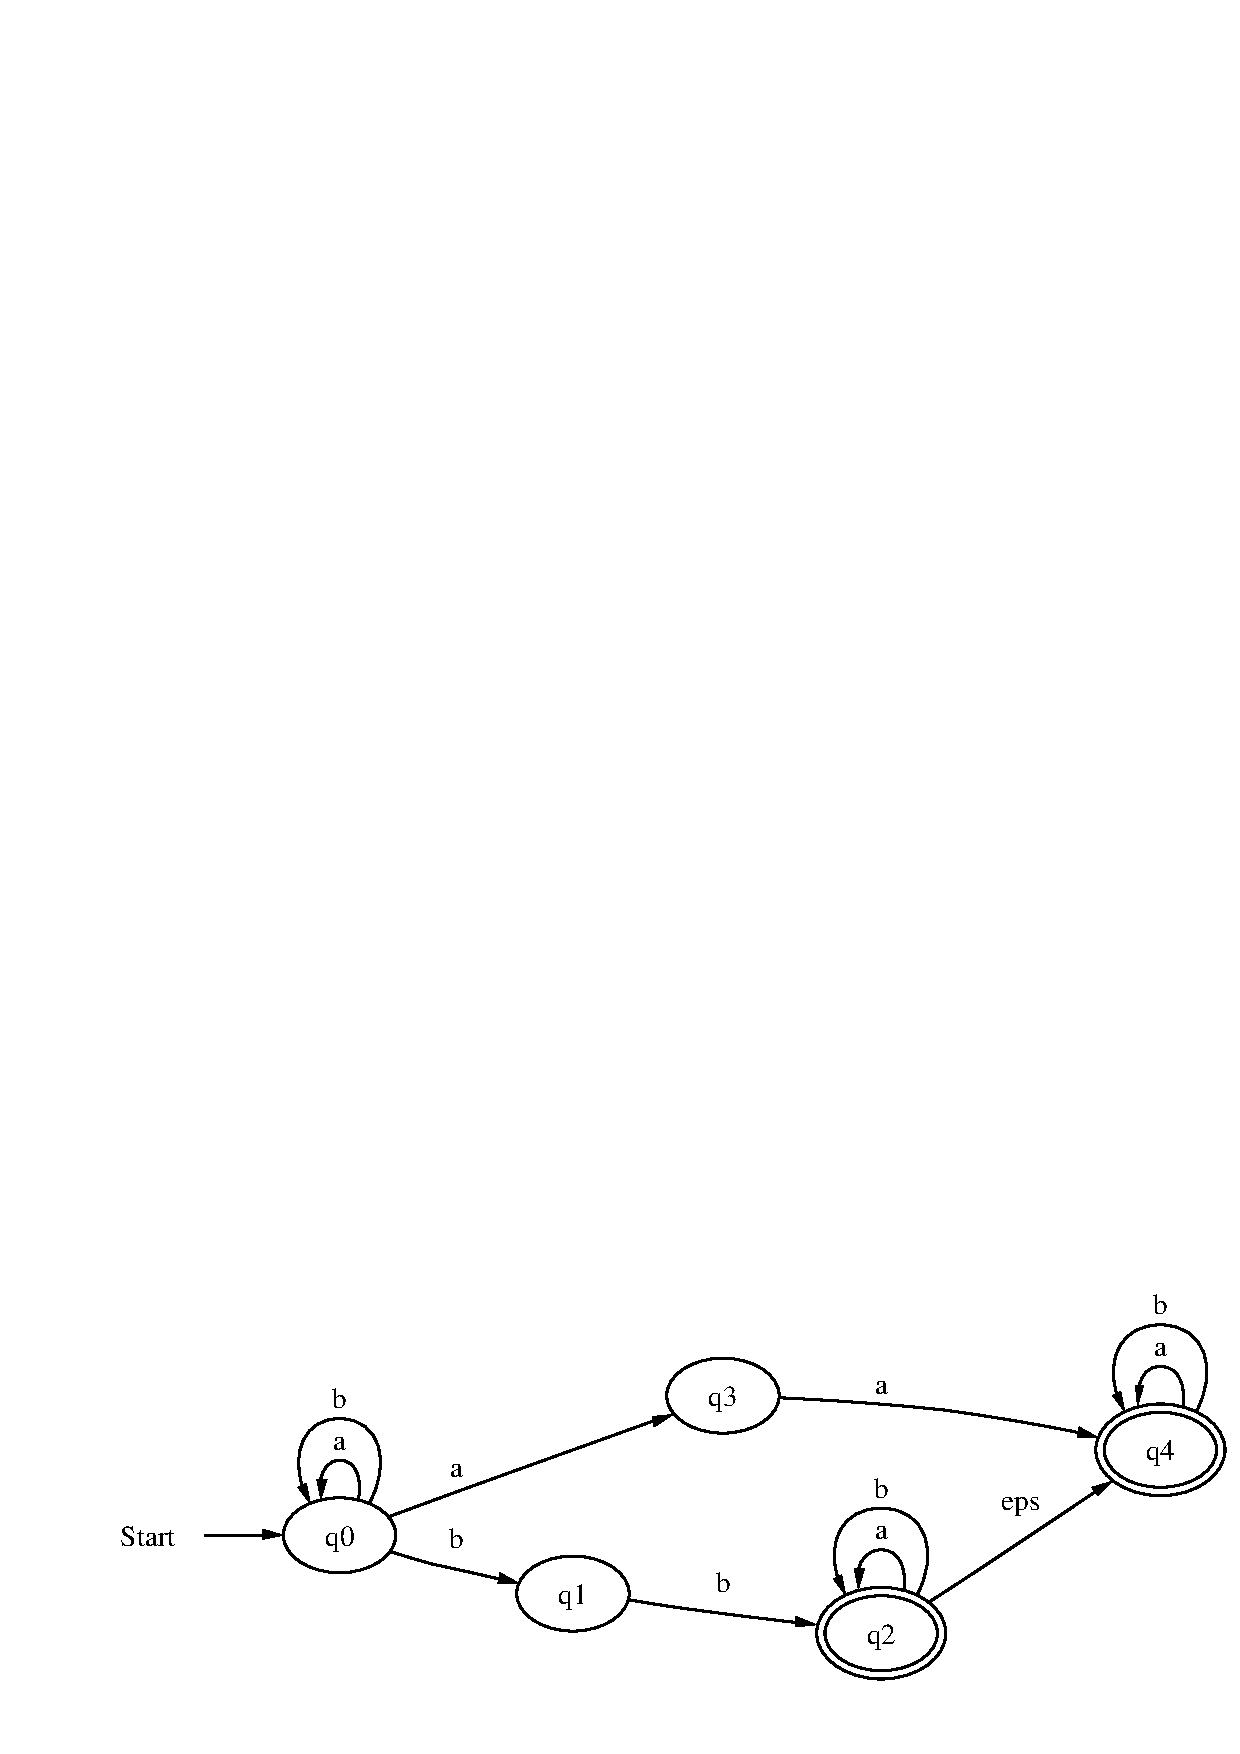
\epsfig{file=nd-fsm, scale=0.95}
\vspace*{\fill}

\tiny \addtocounter{mypage}{1}
\rule{17cm}{1mm}
Pattern Matching \hspace*{\fill} Seite \arabic{mypage}
\end{slide}

%%%%%%%%%%%%%%%%%%%%%%%%%%%%%%%%%%%%%%%%%%%%%%%%%%%%%%%%%%%%%%%%%%%%%%%%

\begin{slide}{}
\normalsize

\begin{center}
  Akzeptierte Sprache
\end{center}
\vspace*{0.5cm}

\footnotesize
\textbf{Gegeben}: Nicht--deterministischer endl. Automat \\[0.3cm]
\hspace*{1.3cm} $F = \langle \Sigma, Z, A, s_0, \mathtt{next}, \mathtt{eps}  \rangle$ 

\textbf{Induktive Definition} der Berechnung eines endlichen Automaten:
\begin{enumerate}
\item $q_1 \stackrel{\varepsilon}{\rightarrow} q_2$ \quad Berechnung mit Label $\varepsilon$ falls 

      $q_2 \in \mathtt{eps}(q_1)$
\item $q_1 \stackrel{c}{\rightarrow} q_2$ \quad Berechnung mit Label $c\in \Sigma$ falls 

      $q_2 \in \mathtt{next}(q_1, c)$
\item $q_0 \stackrel{x_1}{\rightarrow} \cdots \stackrel{x_n}{\rightarrow} q_n \stackrel{x_{n+1}}{\rightarrow} \cdots \stackrel{x_m}{\rightarrow} q_{m}$ \\[0.3cm]
      Berechnung mit Label $vw$ falls 
      \begin{enumerate}
      \item $q_0 \stackrel{x_1}{\rightarrow} \cdots \stackrel{x_n}{\rightarrow} q_n$ Berechnung mit Label $v$
      \item $q_n \stackrel{x_{n+1}}{\rightarrow} \cdots \stackrel{x_m}{\rightarrow} q_{m}$  Berechnung mit Label $w$ ist.
      \end{enumerate}
\end{enumerate}

\textbf{Definition} der \emph{akzeptierten Sprache}: \\[0.3cm]
Ein Wort $w \in \Sigma^*$ ist genau dann in der akzeptierten Sprache $\Ll(F)$, wenn es eine Berechnung \\[0.3cm]
\hspace*{1.3cm} $s_0 \stackrel{x_0}{\rightarrow} \cdots \stackrel{x_n}{\rightarrow} q$ \\[0.3cm]
mit Label $w$ gibt, so dass $q \in F$ ist.

\textbf{Beachte}, dass Berechnung im Start--Zustand $s_0$ startet!

\textbf{Beispiel}: Betrachte letzten Automaten: \\[0.3cm]
\hspace*{1.3cm} $q_0 \stackrel{a}{\rightarrow} q_0 \stackrel{b}{\rightarrow} q_1 \stackrel{b}{\rightarrow} q_2 \stackrel{\varepsilon}{\rightarrow} q_4 \stackrel{a}{\rightarrow}
q_4$ \\[0.3cm]
Berechnung mit Label $abba$, also $abba \in \Ll(F)$.



\vspace*{\fill}
\tiny \addtocounter{mypage}{1}
\rule{17cm}{1mm}
Pattern Matching \hspace*{\fill} Seite \arabic{mypage}
\end{slide}

%%%%%%%%%%%%%%%%%%%%%%%%%%%%%%%%%%%%%%%%%%%%%%%%%%%%%%%%%%%%%%%%%%%%%%%%

\begin{slide}{}
\normalsize

\begin{center}
Berechnung der akzeptierten Sprache
\end{center}
\vspace*{0.5cm}

\footnotesize

Wir erweitern die Funktion $\mathtt{next}$ und $\mathtt{eps}$ zu Funktionen  \\[0.3cm]
\hspace*{1.3cm} $\mathtt{Next}: 2^Z \times \Sigma \rightarrow 2^Z$ \quad und \quad $\mathtt{Eps}: 2^Z \rightarrow 2^Z$

$
\begin{array}{lcl}
 \mathtt{Next}(Q,b) & := & \bigg\{ z \in Z \;|\; \exists q \in Q: z \in \mathtt{next}(q,b) \bigg\} \\[0.5cm]
 \mathtt{Eps}(Q)    & := & Q \cup \bigg\{ z \in Z \;|\; \exists q \in Q: z \in \mathtt{eps}(q) \bigg\}    \\[0.5cm]
\end{array}
$ 

\textbf{Beispiel}: 
\begin{enumerate}
\item $\mathtt{Next}(\{q_0\}, a) = \{q_0, q_3\}$
\item $\mathtt{Next}(\{q_0,q_3\}, a) = \{q_0, q_3, q_4\}$
\item $\mathtt{Eps}(\{q_0\}) = \{q_0\}$
\item $\mathtt{Eps}(\{q_2\}) = \{q_2, q_4\}$
\end{enumerate}


Wir erweitern die Funktion \texttt{Next} induktiv auf Worte $w$ zu einer Funktion \\[0.3cm]
\hspace*{1.3cm} $\texttt{Next}^*: 2^Z \times \Sigma^* \rightarrow 2^Z$
\begin{enumerate}
\item $\texttt{Next}^*(Q, \varepsilon)\quad :=\; \mathtt{Eps}(Q)$
\item $\mathtt{Next}^*(Q, bw) \;:=\; \mathtt{Next}^*\Bigg(\; \mathtt{Next}\bigg(\,\mathtt{Eps}(Q),\,b\,\bigg),\; w\;\Bigg)$
\end{enumerate}

\textbf{Beispiel}:
\begin{enumerate}
\item $\mathtt{Next}^*(\{q_0\}, aa) = \{q_0, q_3, q_4\}$
\item $\mathtt{Next}^*(\{q_0\}, abba) = \{q_0, q_2, q_3, q_4\}$
\end{enumerate}

\textbf{Satz}: Ist $F$ nicht--determ. Automat, so gilt: \\[0.3cm]
\hspace*{1.3cm} $\Ll(F) \;=\; \bigg\{ w \in \Sigma^* \;|\; \mathtt{Next}^*(\{s_0\},w) \cap F \not= \emptyset \bigg\}$

\vspace*{\fill}
\tiny \addtocounter{mypage}{1}
\rule{17cm}{1mm}
Pattern Matching \hspace*{\fill} Seite \arabic{mypage}
\end{slide}

%%%%%%%%%%%%%%%%%%%%%%%%%%%%%%%%%%%%%%%%%%%%%%%%%%%%%%%%%%%%%%%%%%%%%%%%

\begin{slide}{}
\normalsize

\begin{center}
Potenz--Mengen--Konstruktion
\end{center}
\vspace*{0.5cm}

\footnotesize
\textbf{Gegeben}: Nicht--deterministische FSM \\[0.3cm]
\hspace*{1.3cm} $F_{nd} = \langle \Sigma, Z, A, s_0, \mathtt{next}, \mathtt{eps}  \rangle$ 

\textbf{Gesucht}: Deterministische FSM \\[0.3cm]
\hspace*{1.3cm} $F_{det} = \langle \Sigma, \cl{Z}, \cl{A}, S_0, \NS  \rangle$  \\[0.3cm]
mit $\Ll(F_{det}) = \Ll(F_{nd})$

\textbf{Definition}:
\begin{enumerate}
\item $\cl{Z} := 2^Z$
\item $\cl{A} := \bigg\{ M \in 2^Z \;|\; M \cap F \not = \emptyset \}$
\item $S_0 := \{s_0\}$
\item $\NS(Q) := \mathtt{Eps}\Bigg(\; \mathtt{Next}\bigg(\, \mathtt{Eps}(Q), b \,\bigg) \;\Bigg)$
\end{enumerate}
Zahl der Zust"ande: $|\cl{Z}| = 2^{|Z|}$: sehr gro\3!

\textbf{Satz}:  $\Ll(F_{det}) = \Ll(F_{nd})$

\textbf{Beobachtung}: Nicht--deterministische Automaten sind \\
nicht m"achtiger als deterministische Automaten.

\vspace*{\fill}
\tiny \addtocounter{mypage}{1}
\rule{17cm}{1mm}
Pattern Matching \hspace*{\fill} Seite \arabic{mypage}
\end{slide}

%%%%%%%%%%%%%%%%%%%%%%%%%%%%%%%%%%%%%%%%%%%%%%%%%%%%%%%%%%%%%%%%%%%%%%%%

\begin{slide}{}
\normalsize

\begin{center}
"Ubersetzung von regul"aren Ausdr"ucken in
nicht--deterministische FSMs
\end{center}
\vspace*{0.5cm}

\footnotesize
Wir definieren f"ur jeden regul"aren Ausdruck $r$ eine
nicht--deterministische FSM durch Induktion "uber $r$

Konstruktions--Invarianten:
\begin{enumerate}
\item Menge der akzeptierenden Zust"ande ein--elementig
\item $|\mathtt{eps}(q)|    \leq 2$
\item $|\bigcup\limits_{b\in\Sigma} \mathtt{next}(q,b)| \leq 1$
\item $\mathtt{eps}(q) = \emptyset \;\vee\; \forall b\in\Sigma:\mathtt{next}(q,b) = \emptyset$
\end{enumerate}
\textbf{Induktive Definition}:
\begin{enumerate}
\item $r = \emptyset$: 

            \hspace*{1.3cm} 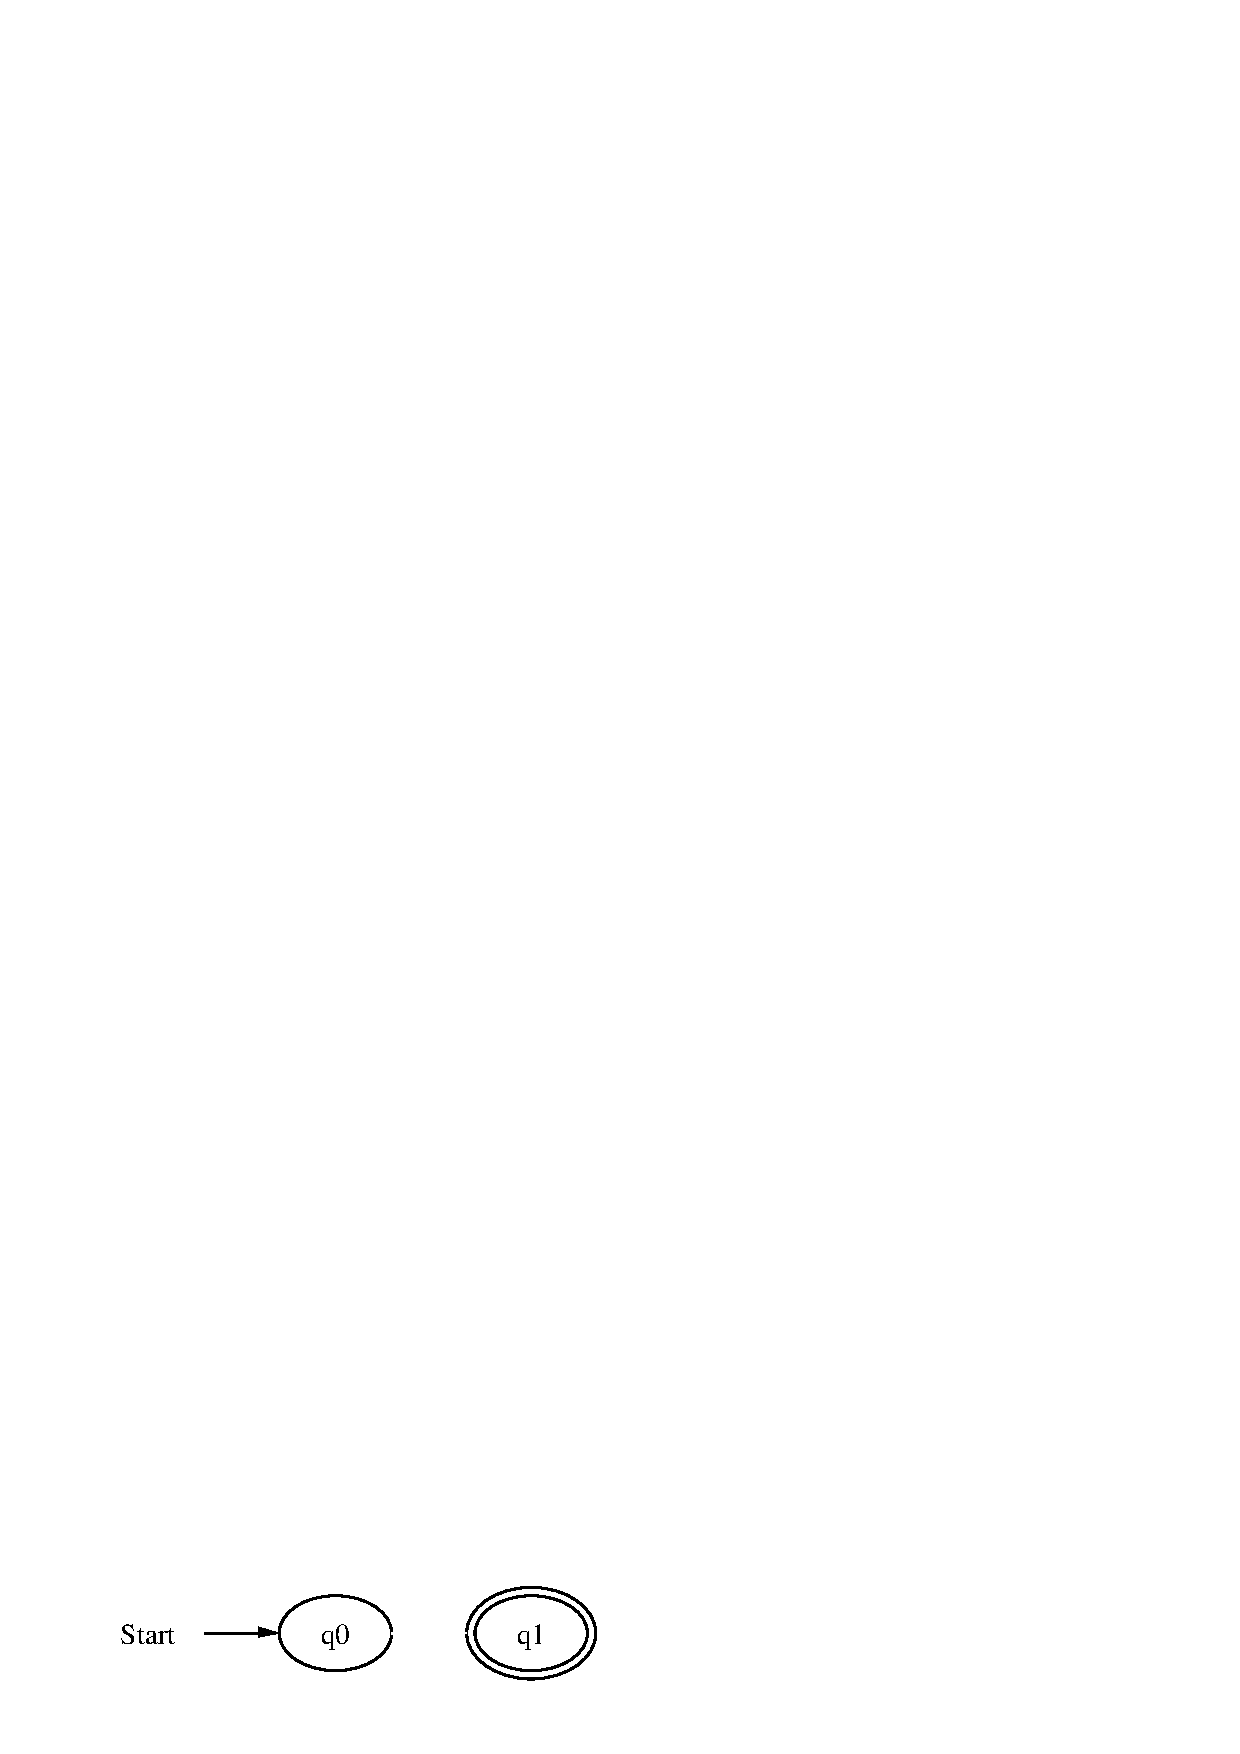
\epsfig{file=empty}
\item $r = \varepsilon$: 

            \hspace*{1.3cm} 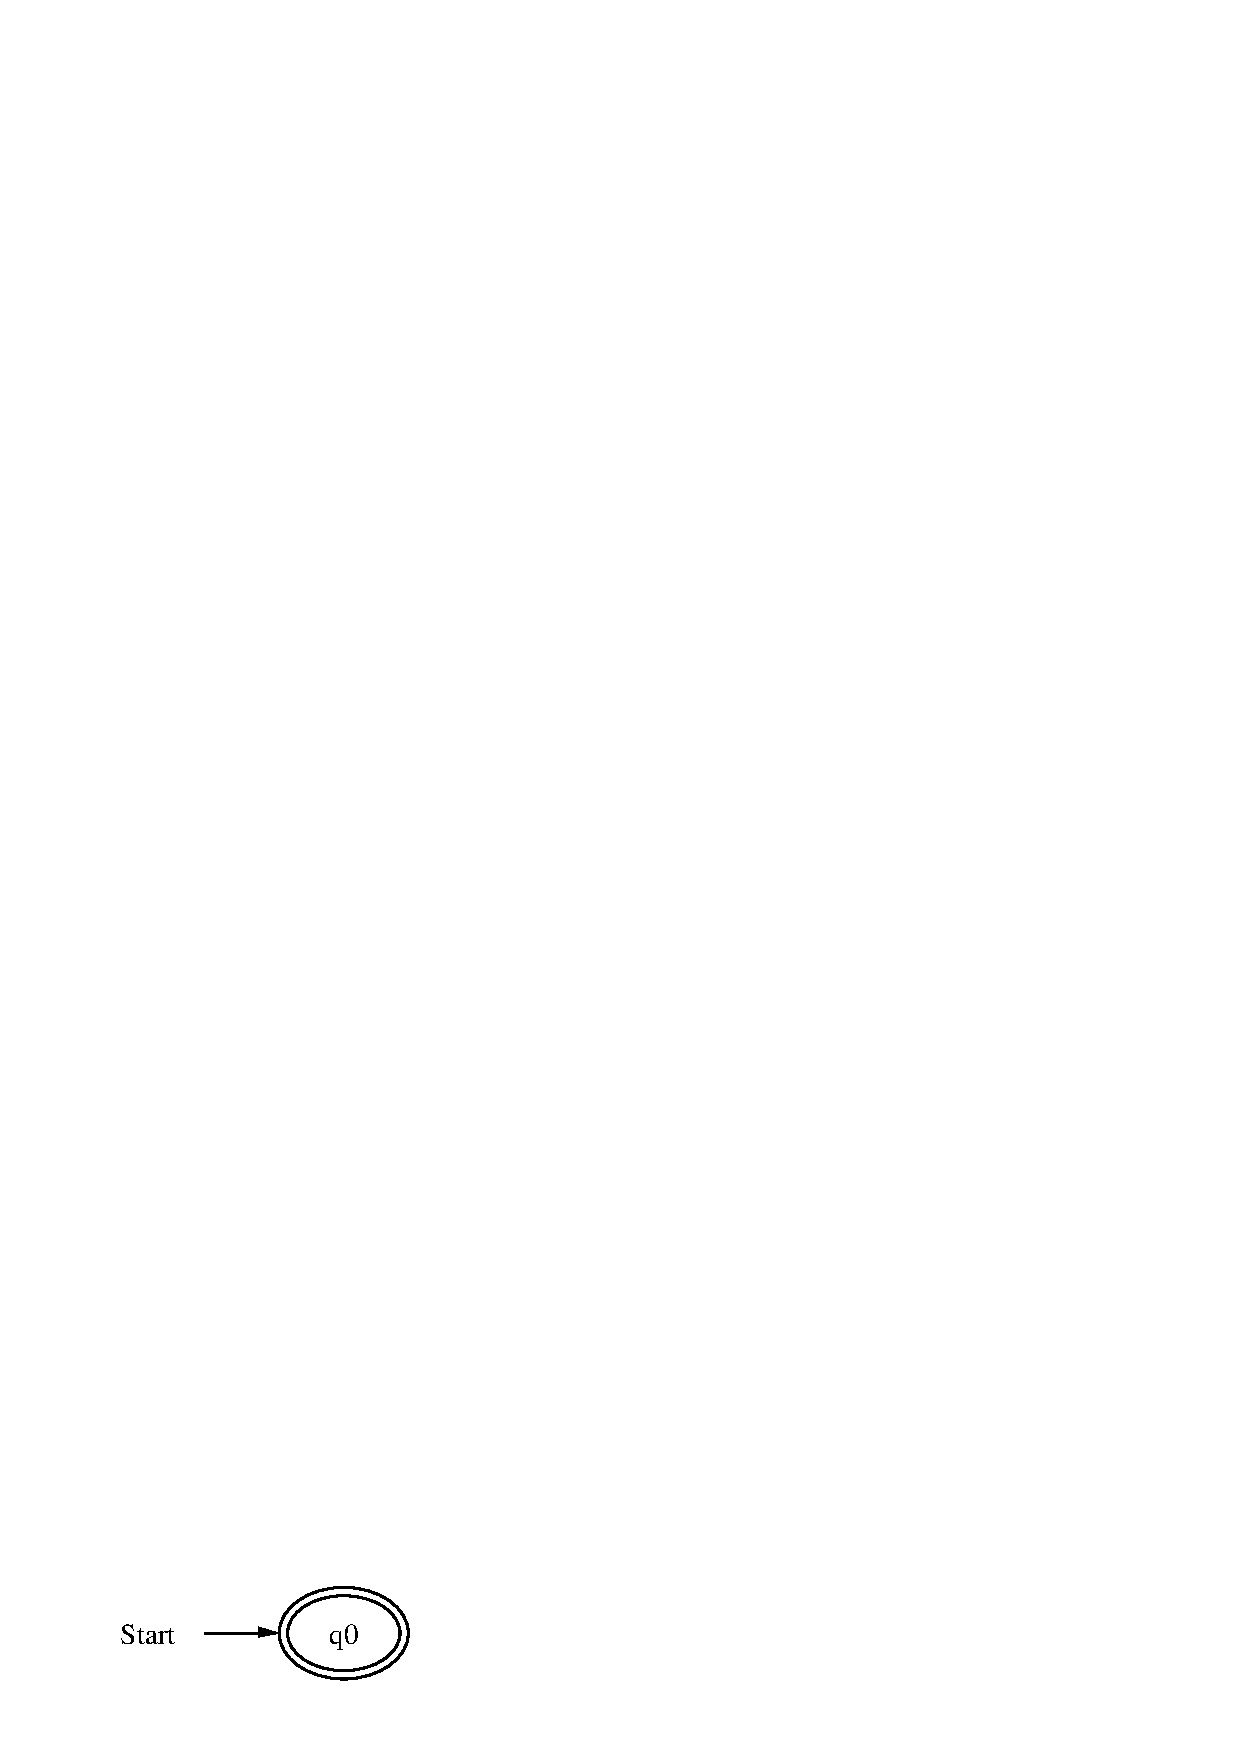
\epsfig{file=epsilon-fsm}
\item $r = b$ mit $b \in \Sigma$: 

            \hspace*{1.3cm} 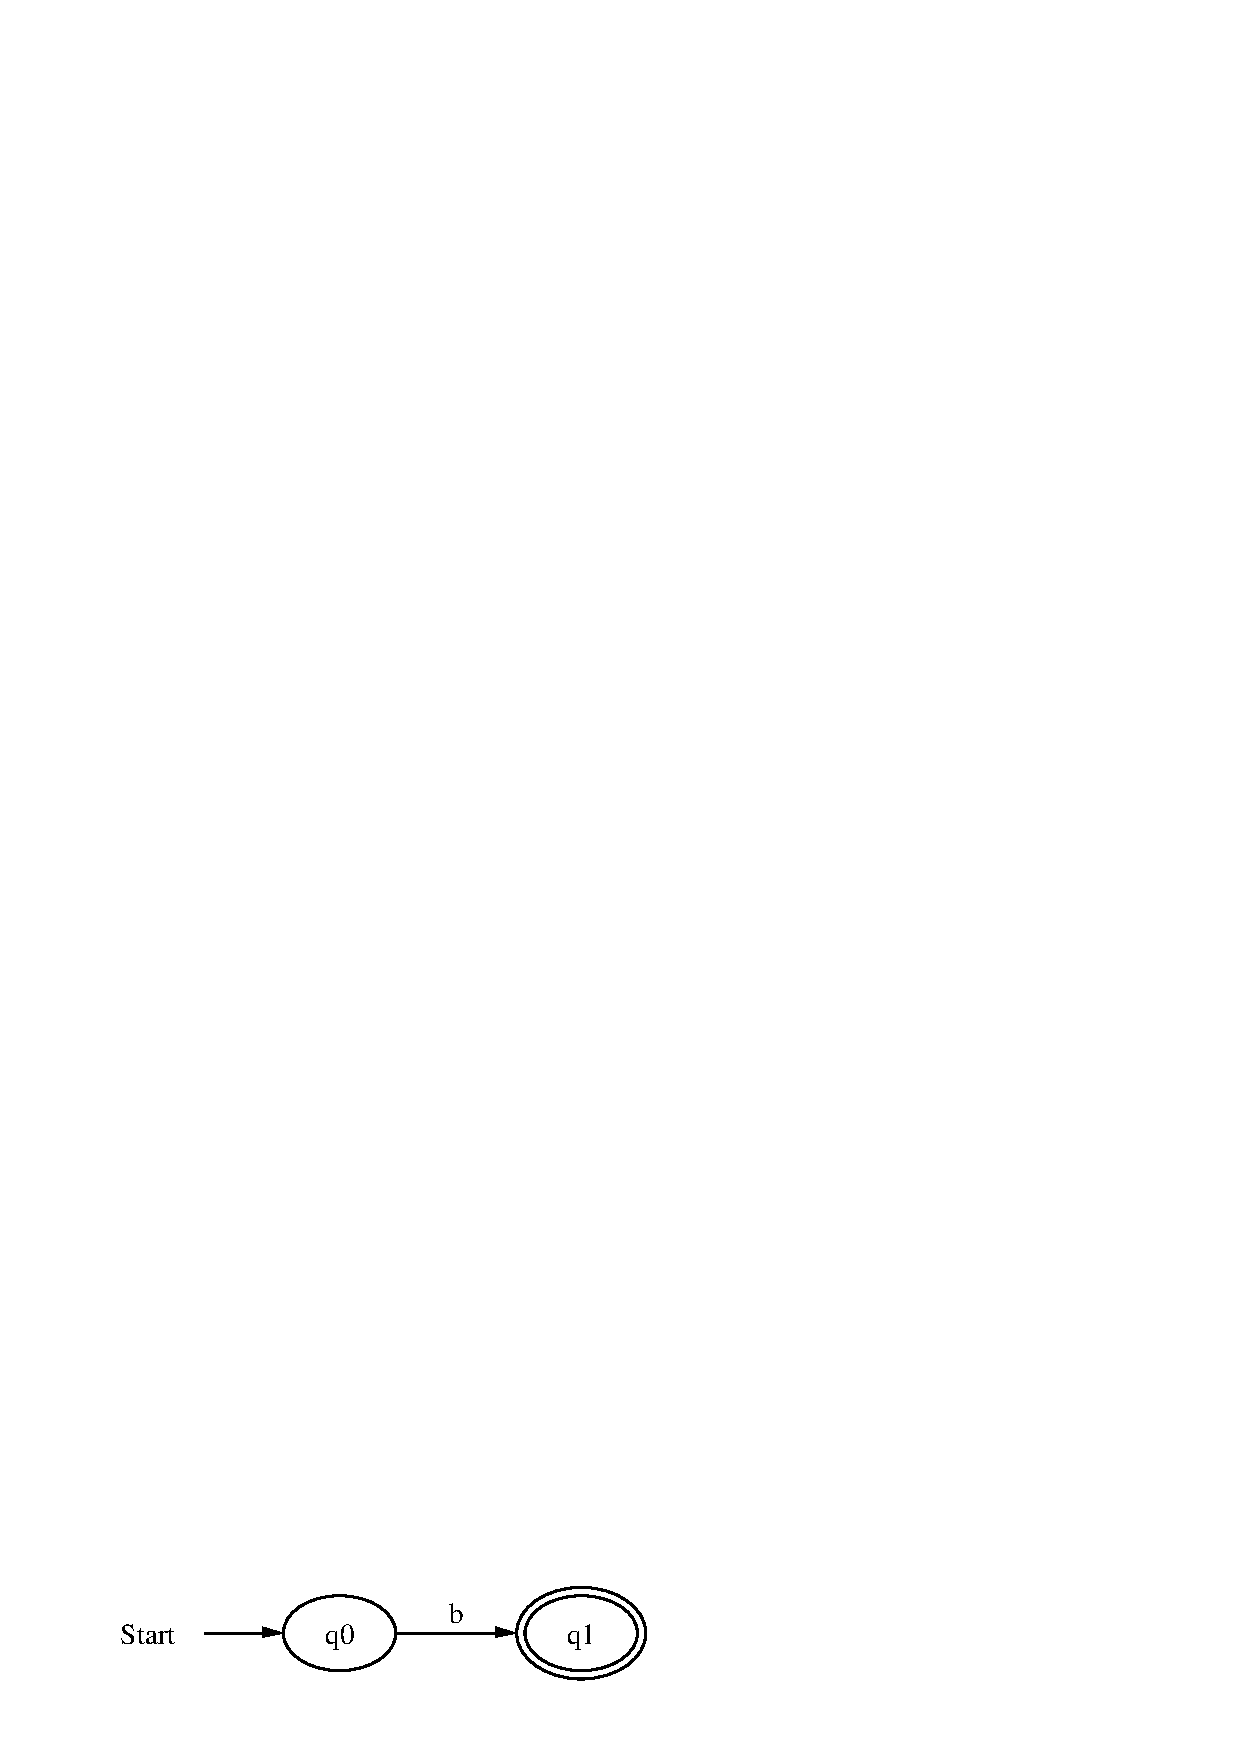
\epsfig{file=letter}
      \vspace*{0.5cm}
\end{enumerate}


\vspace*{\fill}
\tiny \addtocounter{mypage}{1}
\rule{17cm}{1mm}
Pattern Matching \hspace*{\fill} Seite \arabic{mypage}
\end{slide}

%%%%%%%%%%%%%%%%%%%%%%%%%%%%%%%%%%%%%%%%%%%%%%%%%%%%%%%%%%%%%%%%%%%%%%%%

\begin{slide}{}
\normalsize

\begin{center}
\texttt{RegExp} $\mapsto$ FSM (Fortsetzung)
\end{center}
\vspace*{0.5cm}

\footnotesize
Nach IV seien FSMs f"ur $r_1$ und $r_2$  wie folgt gegeben:
\begin{enumerate}
\item $r_1$: \vspace*{-0.7cm}

      \hspace*{1.3cm} 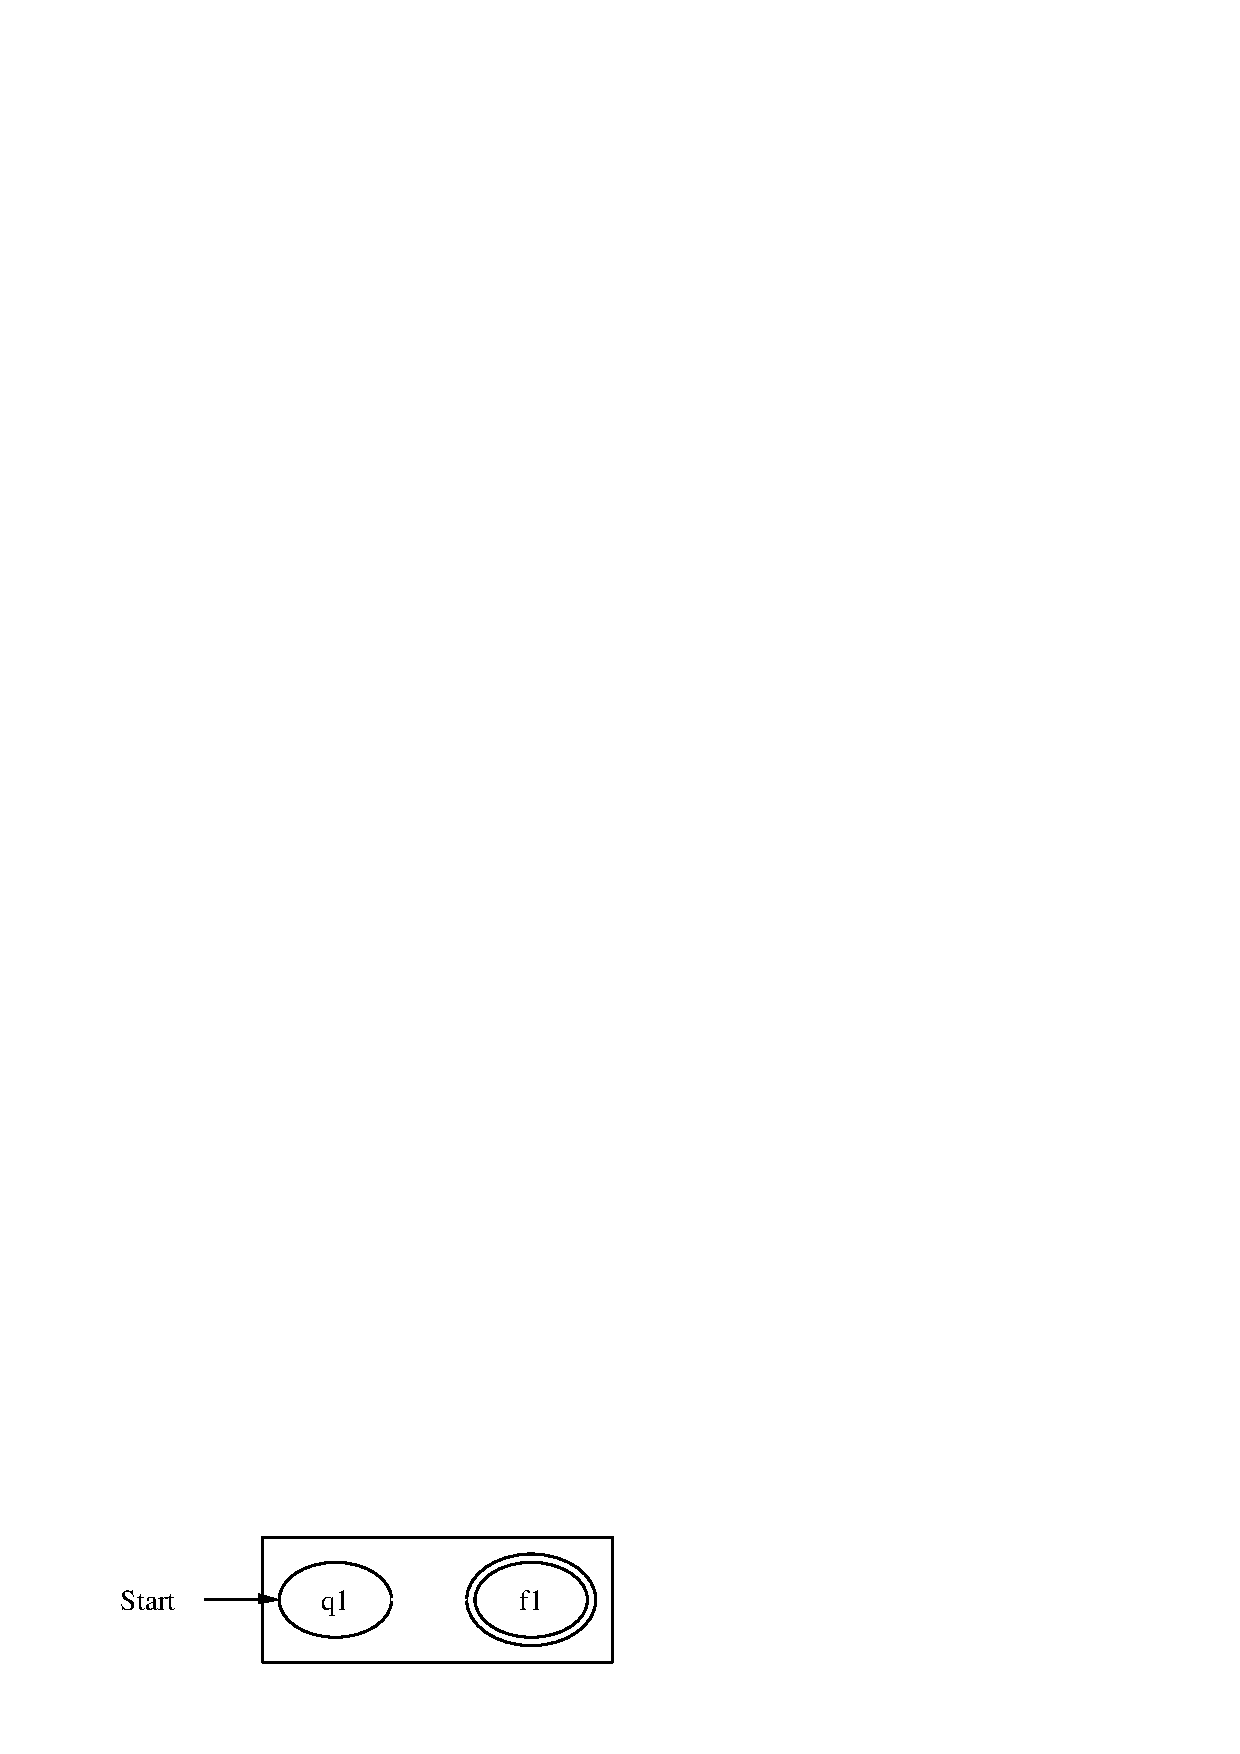
\epsfig{file=r1}
\item $r_2$: \vspace*{-0.7cm}

      \hspace*{1.3cm} 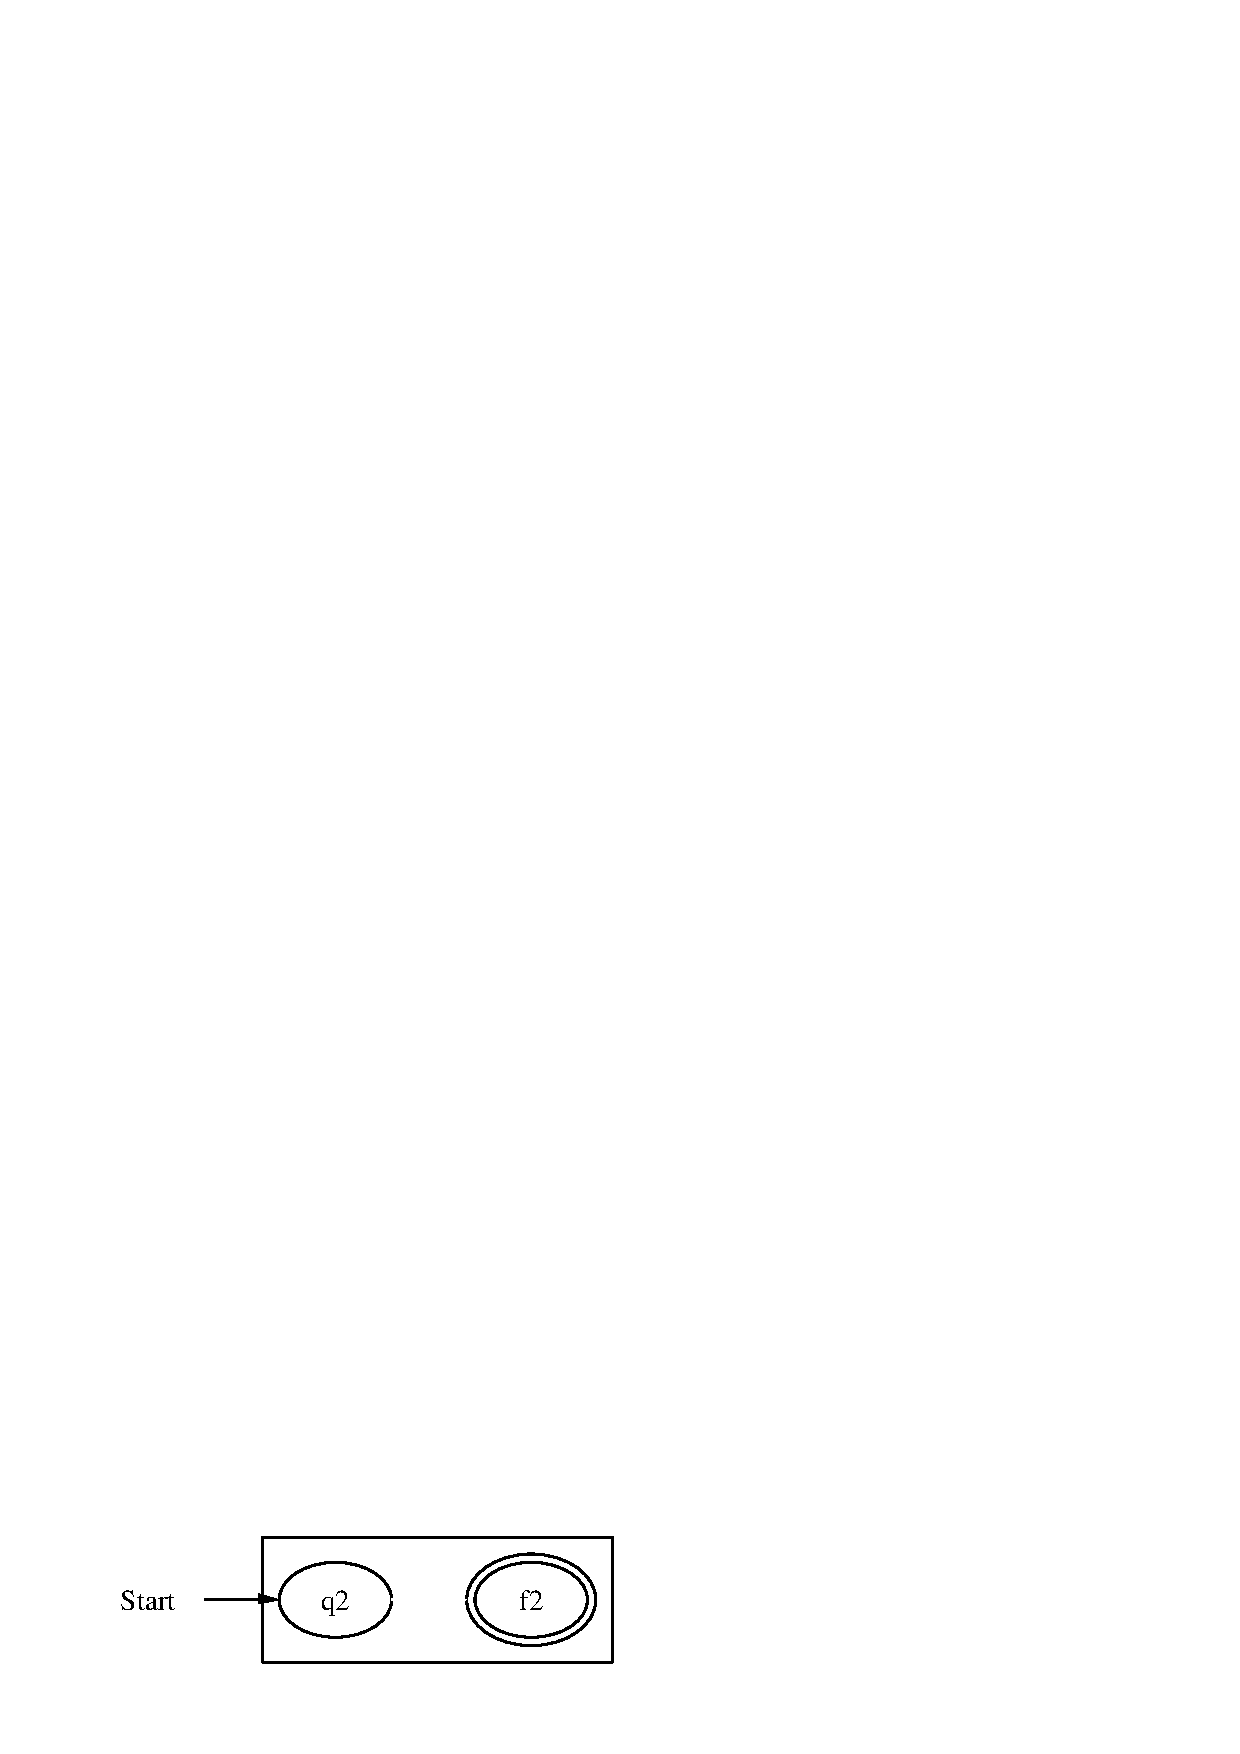
\epsfig{file=r2}
\end{enumerate}
Fortsetzung der induktiven Definition:
\begin{enumerate}
\item[4.] $r = r_1r_2$ 

      \hspace*{-2cm} 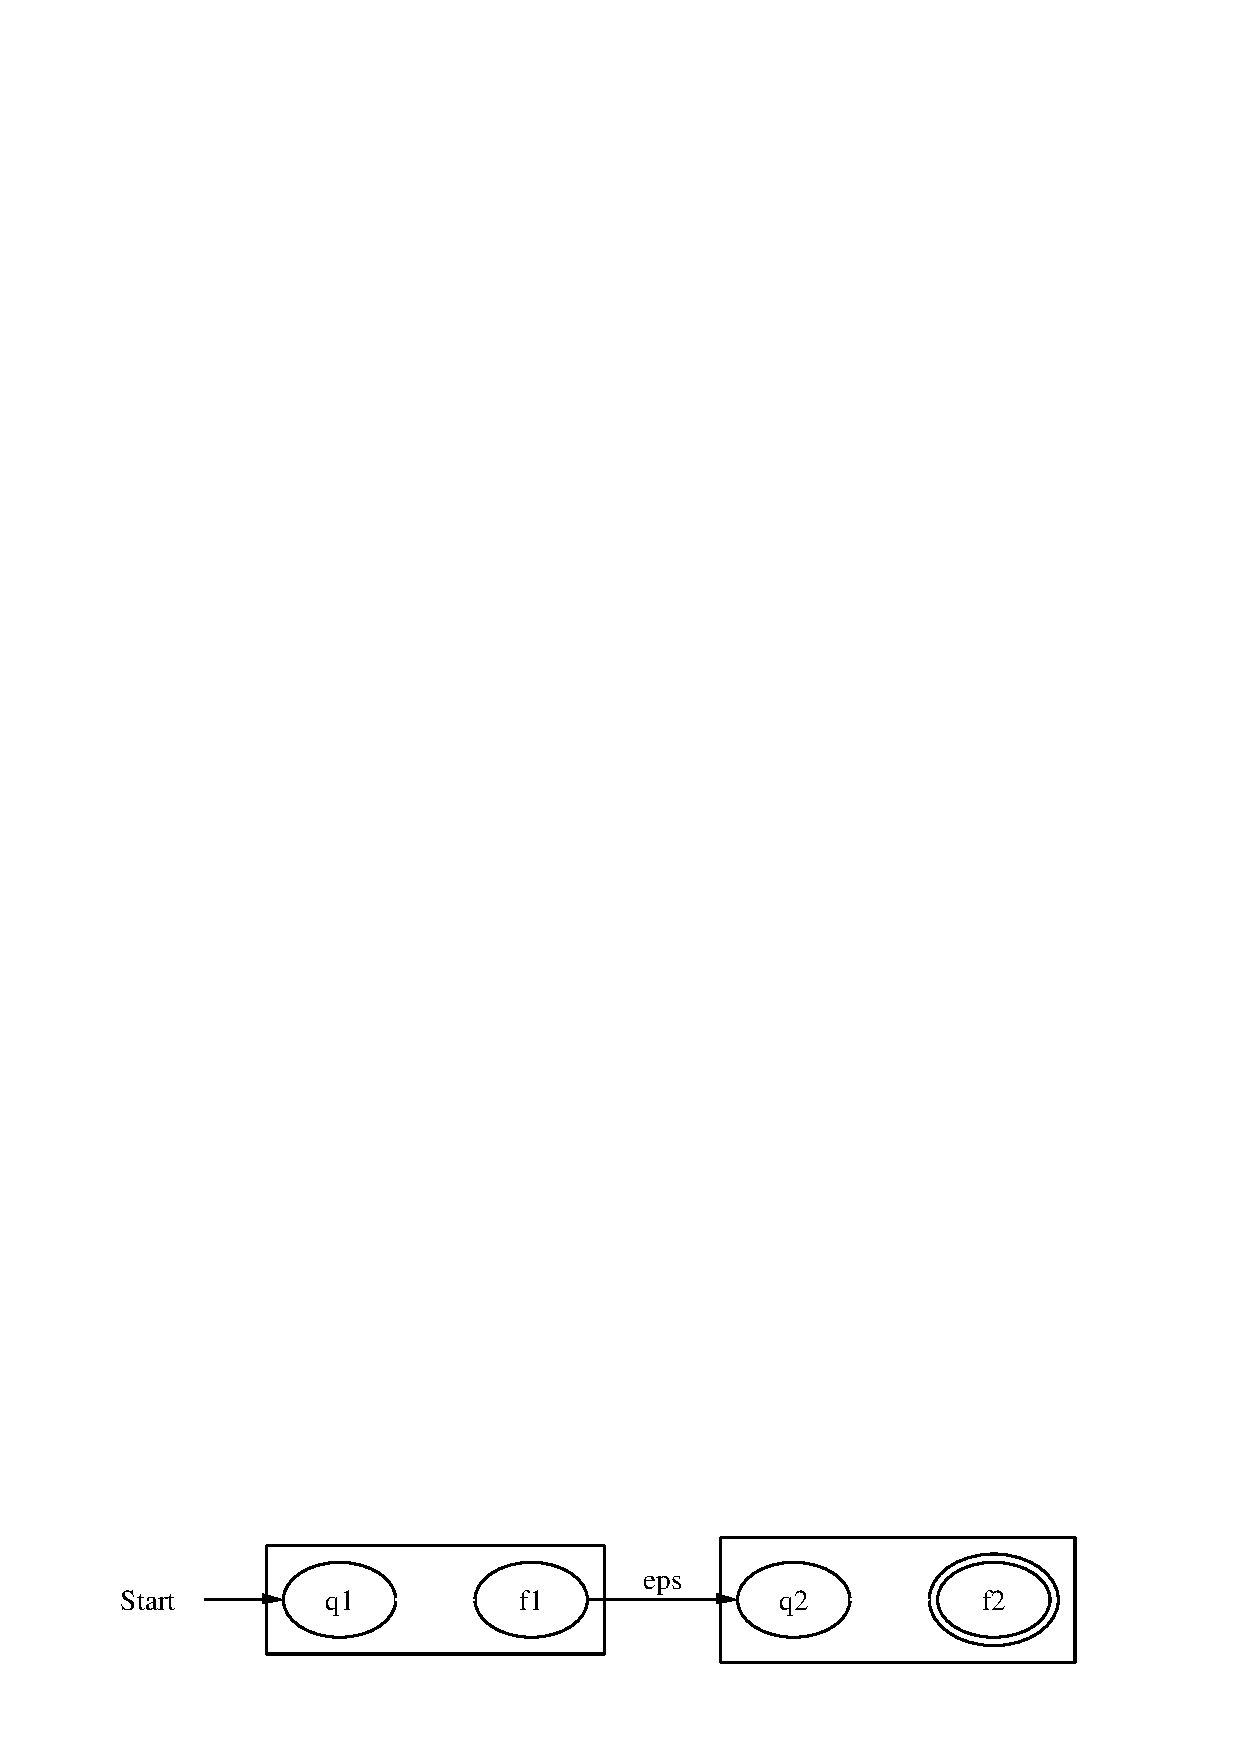
\epsfig{file=concat}
\item[5.] $r = r_1 + r_2$

      \hspace*{-2cm} 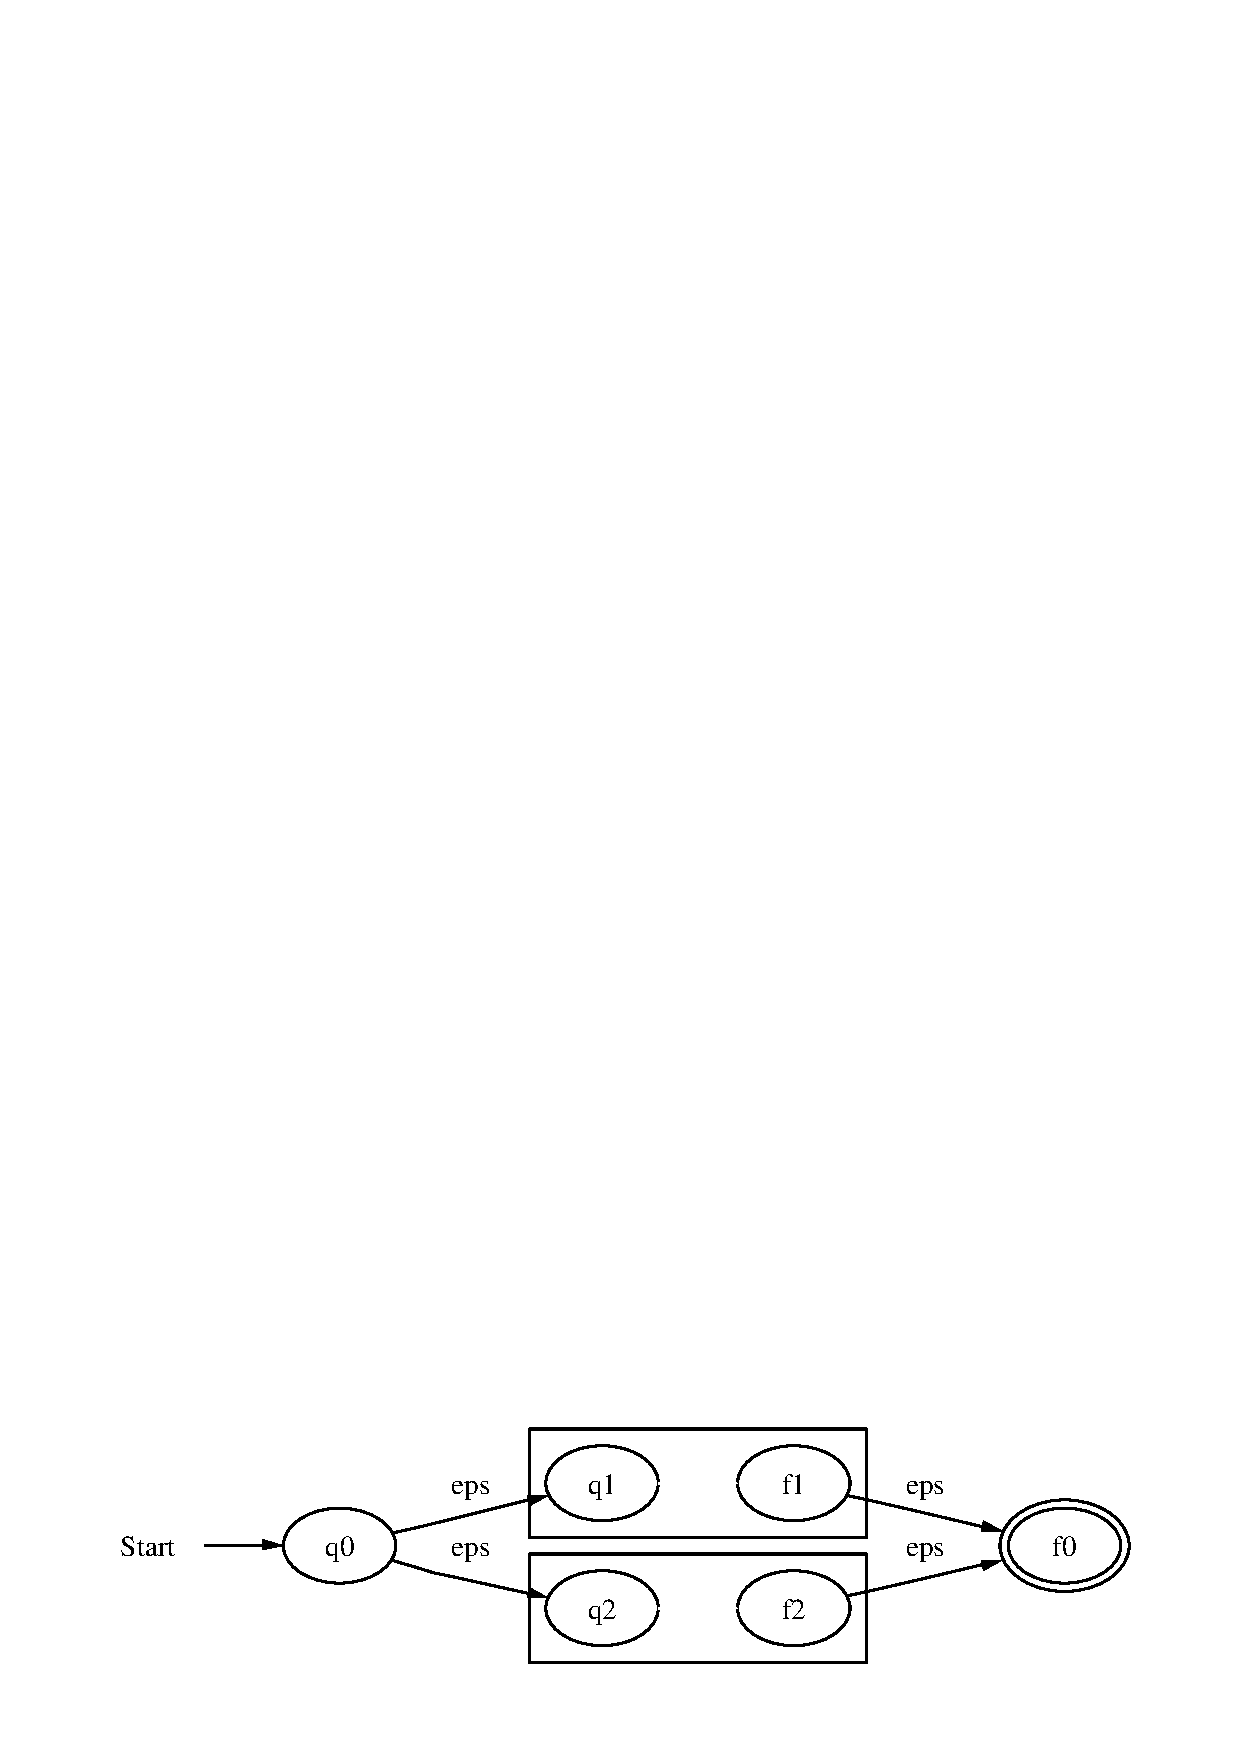
\epsfig{file=alternation}
\end{enumerate}


\vspace*{\fill}
\tiny \addtocounter{mypage}{1}
\rule{17cm}{1mm}
Pattern Matching \hspace*{\fill} Seite \arabic{mypage}
\end{slide}

%%%%%%%%%%%%%%%%%%%%%%%%%%%%%%%%%%%%%%%%%%%%%%%%%%%%%%%%%%%%%%%%%%%%%%%%

\begin{slide}{}
\normalsize

\begin{center}
Konstruktion der FSM f"ur $r_1^*$
\end{center}
\vspace*{0.5cm}

\footnotesize
Nach IV sei FSM f"ur $r_1$ gegeben durch

\hspace*{1.3cm} 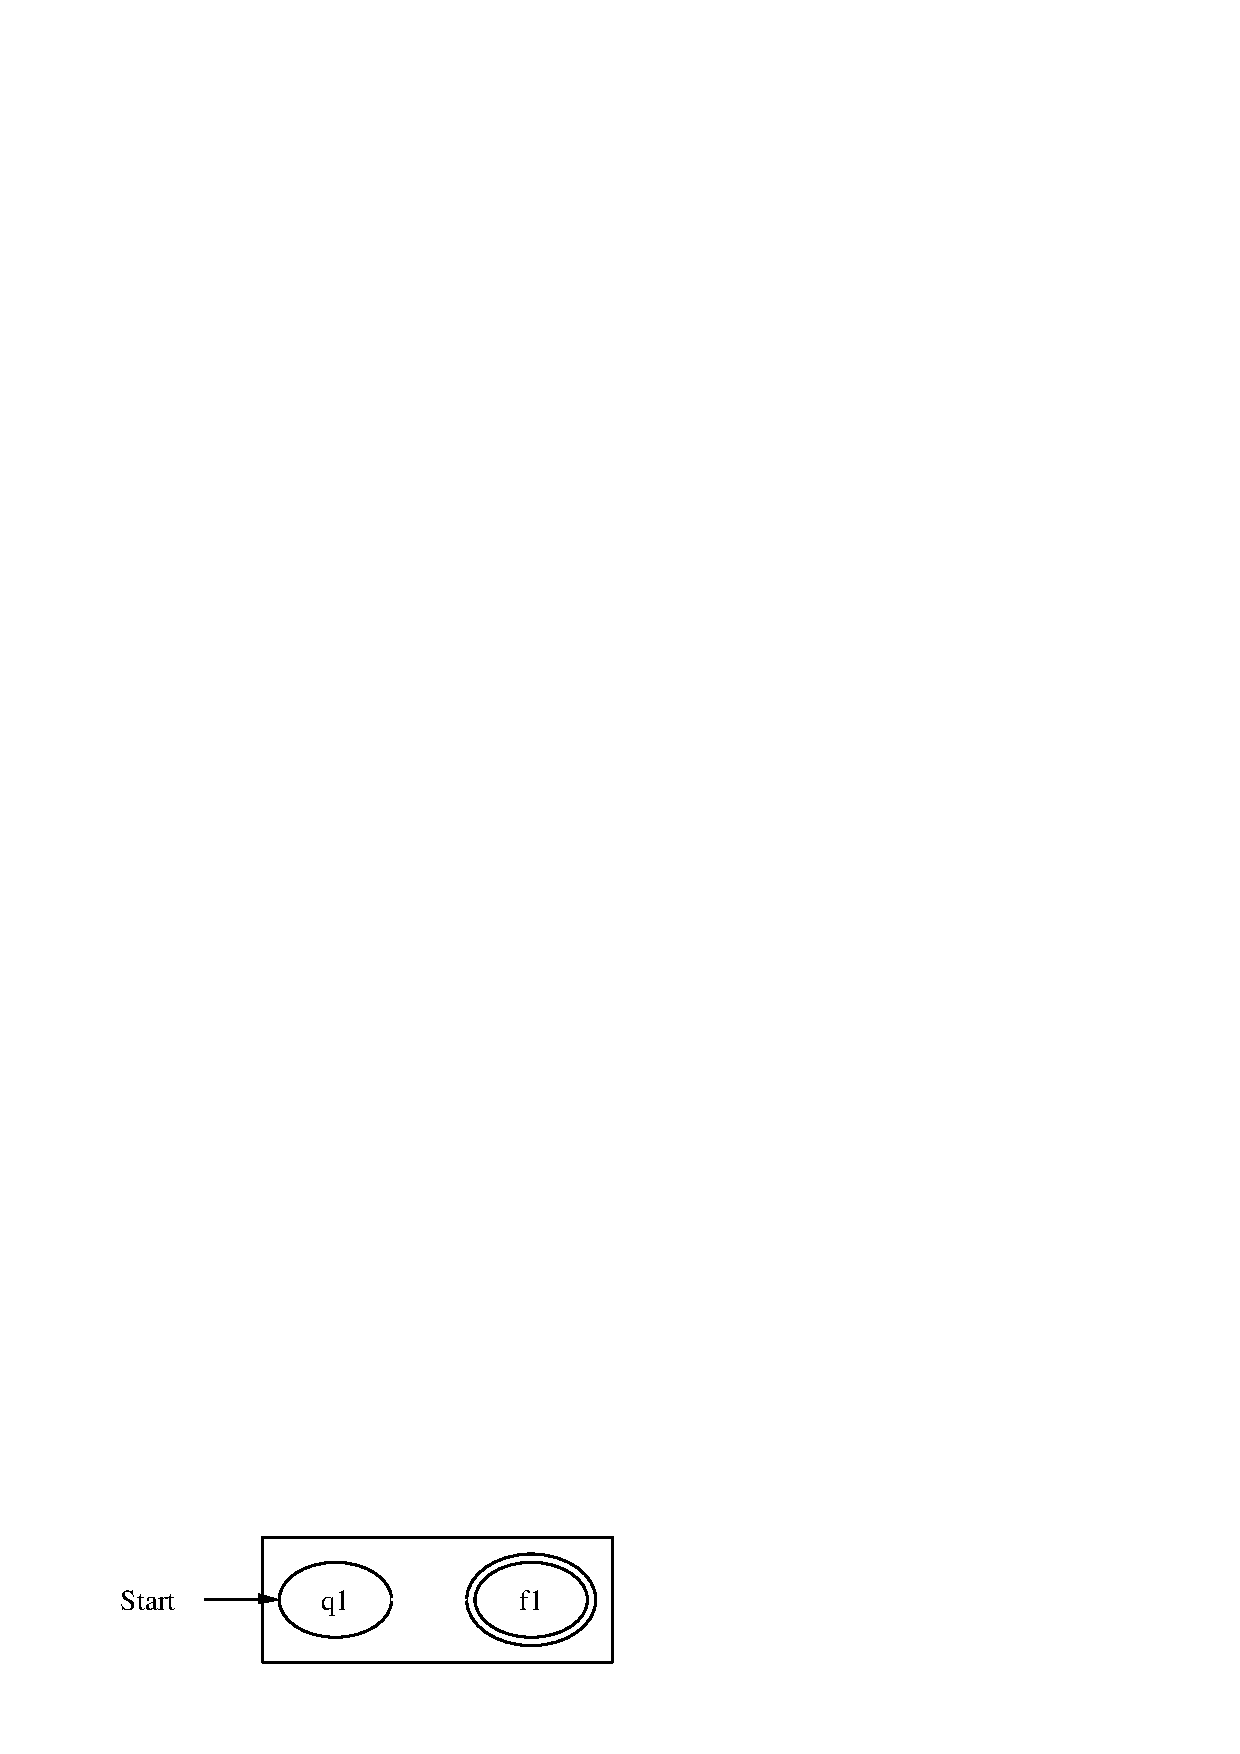
\epsfig{file=r1}

Fortsetzung der induktiven Definition
\begin{enumerate}
\item[6.] $r = r_1^*$ \vspace*{-1.5cm}

          \hspace*{5.3cm} 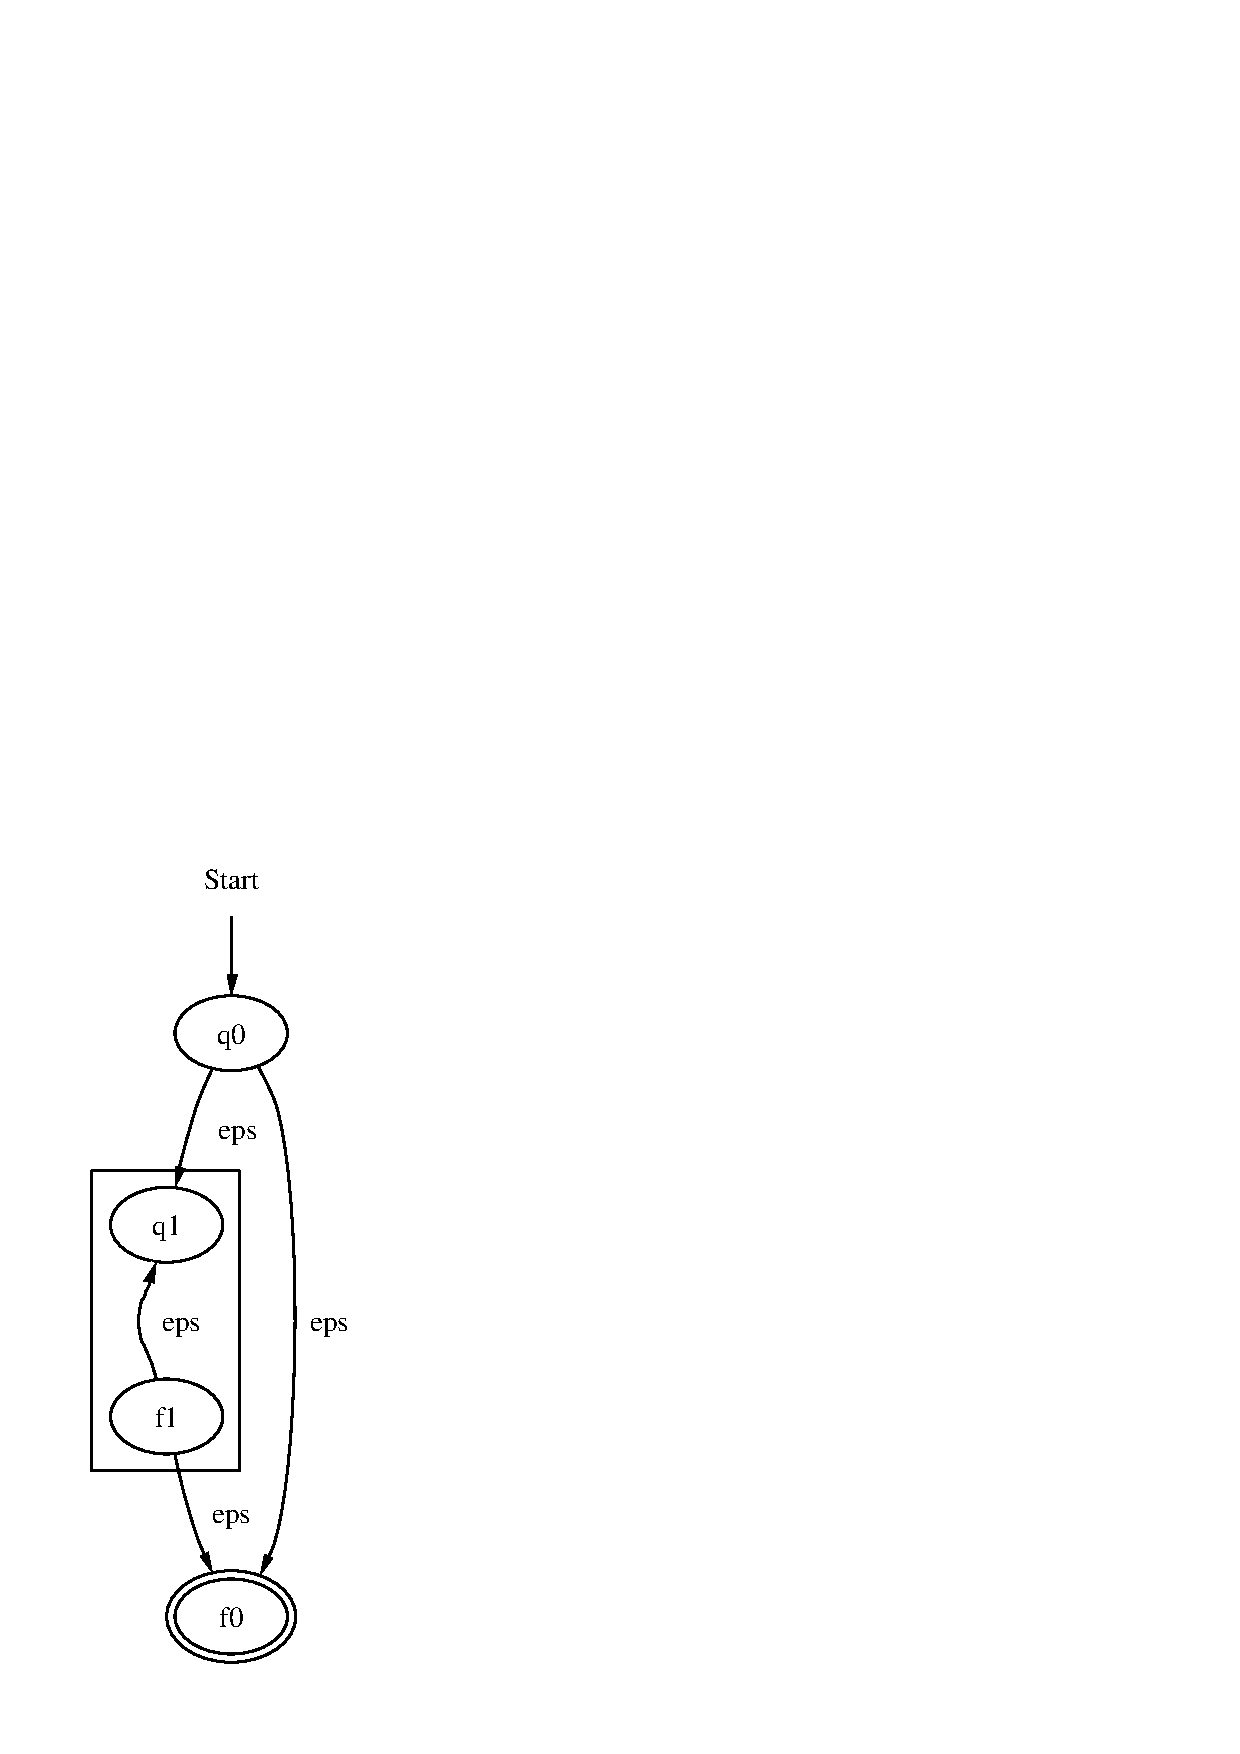
\epsfig{file=closure} 
\end{enumerate}

\vspace*{\fill}
\tiny \addtocounter{mypage}{1}
\rule{17cm}{1mm}
Pattern Matching \hspace*{\fill} Seite \arabic{mypage}
\end{slide}

%%%%%%%%%%%%%%%%%%%%%%%%%%%%%%%%%%%%%%%%%%%%%%%%%%%%%%%%%%%%%%%%%%%%%%%%

\begin{slide}{}
\normalsize

\begin{center}
Beispiel: $(a|b)^{*}abb$
\end{center}

\footnotesize
\hspace*{3.3cm} 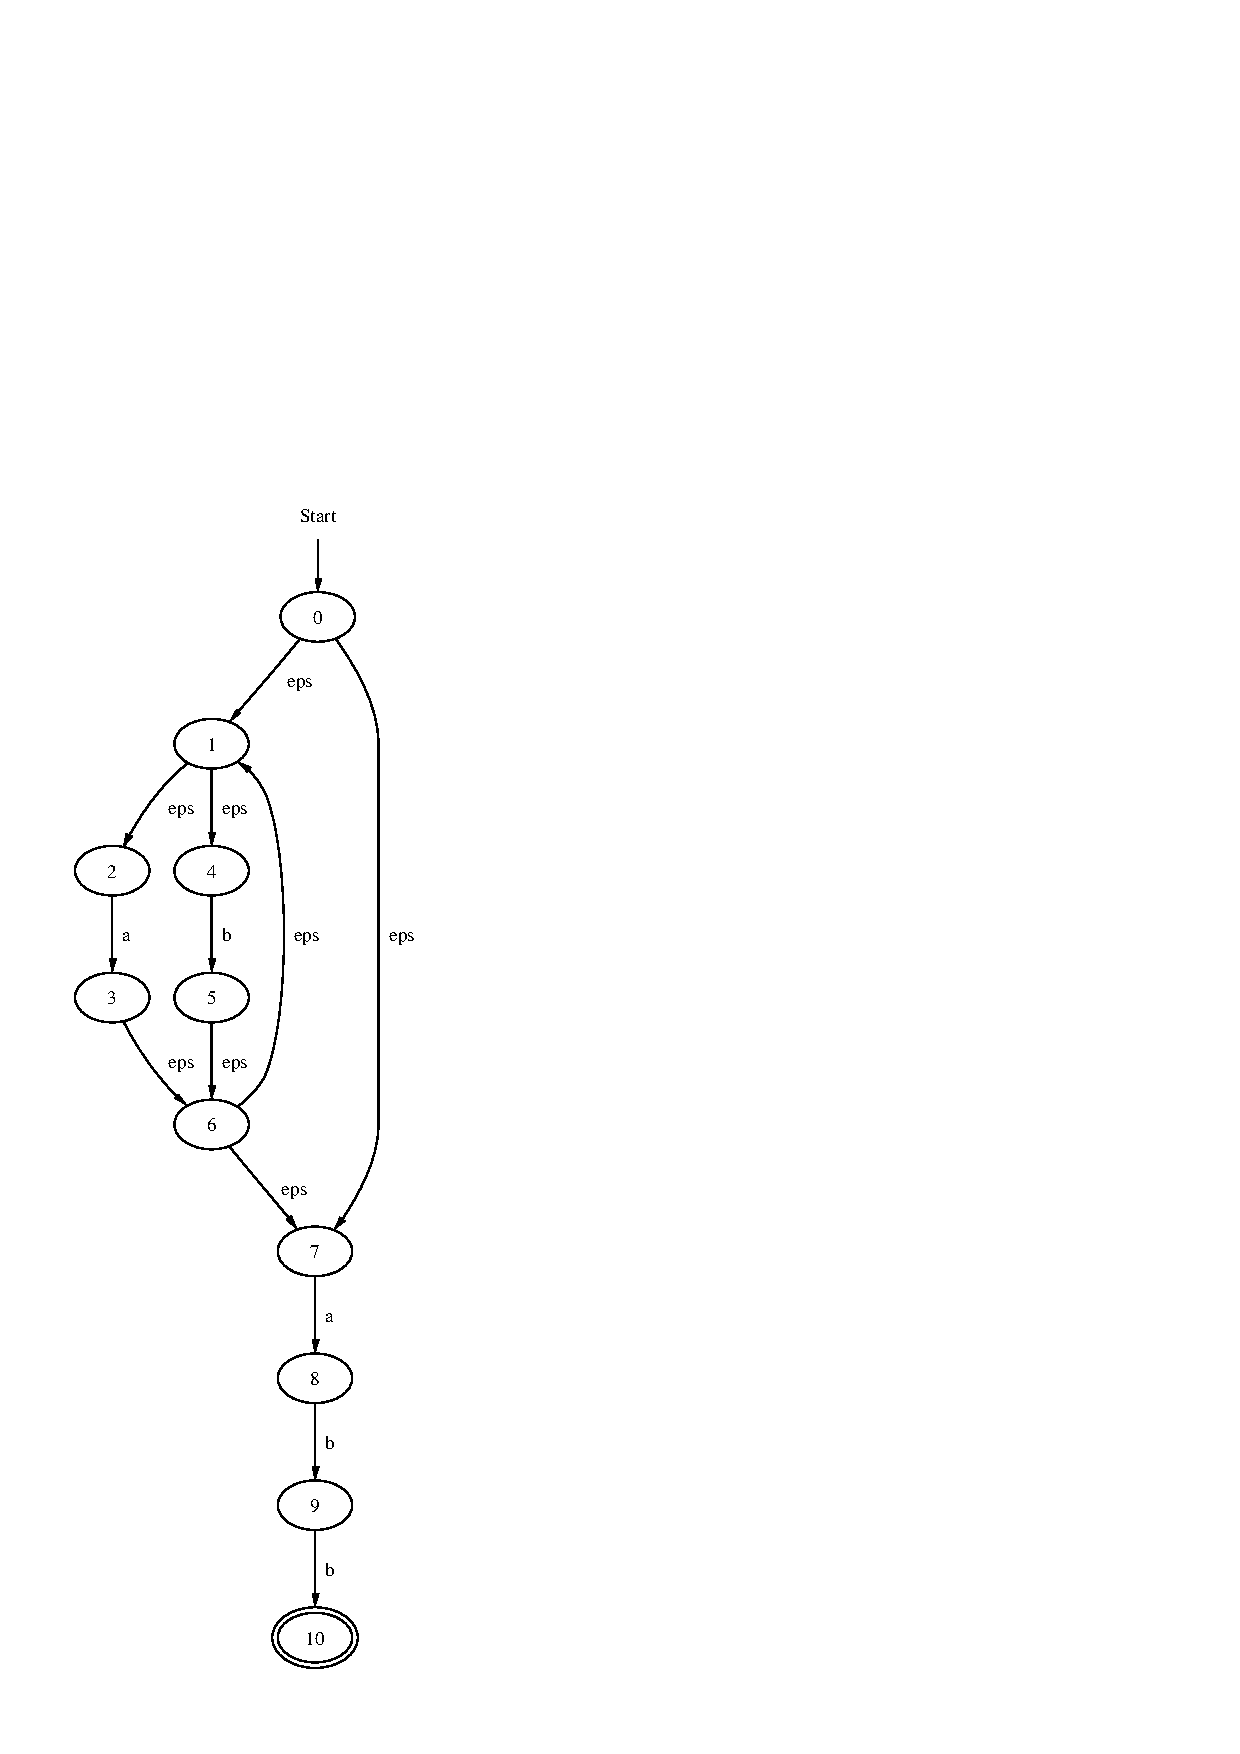
\epsfig{file=example-regexp}

\vspace*{\fill}
\tiny \addtocounter{mypage}{1}
\rule{17cm}{1mm}
Pattern Matching \hspace*{\fill} Seite \arabic{mypage}
\end{slide}

%%%%%%%%%%%%%%%%%%%%%%%%%%%%%%%%%%%%%%%%%%%%%%%%%%%%%%%%%%%%%%%%%%%%%%%%%

\begin{slide}{}
\normalsize

\begin{center}
Simulation nicht--deterministischer FSMs
\end{center}
\vspace*{0.5cm}

\footnotesize
\textbf{Problem}: Gr"o\3e  Potenz--Mengen--Konstruktion: $2^{|Z|}$

\textbf{L"osung}: \emph{Simulation} der Potenz--Mengen--Konstruktion

Repr"asentation einer FSM
\begin{enumerate}
\item Anzahl der Zust"ande: \texttt{numberStates}
\item Codierung der Zust"ande als Zahlen: \\[0.3cm]
      \hspace*{1.3cm}  $0, \cdots, \mathtt{numberStates}-1$
\item Feld von Symbolen: \texttt{symbol[numberStates]} 
\item Feld von Folge--Zust"anden: \texttt{next1[numberStates]} 
\item Feld von Folge--Zust"anden: \texttt{next2[numberStates]} 
\end{enumerate}
Bedeutung dieser Felder:
\begin{enumerate}
\item $j \in \texttt{next}(i, c) \rightarrow \mathtt{symbol}[i] = c$
\item $\bigg(\forall c \in \Sigma:  \texttt{next}(i, c) = \emptyset \bigg) \rightarrow \mathtt{symbol}[i] = 0$
\item $j \in \mathtt{next}(i,c) \rightarrow \mathtt{next1}[i] = j$
\item $j \in \mathtt{eps}(i) \rightarrow \mathtt{next1}[i] = j \vee \mathtt{next2}[i] = j$
\end{enumerate}

C--Daten--Struktur
\begin{verbatim}
typedef struct {
    unsigned  numberStates; // number of states
    char*     symbol;       // array of characters
    unsigned* next1;        // possible next state
    unsigned* next2;        // possible next state
} FSM;
\end{verbatim}


\vspace*{\fill}
\tiny \addtocounter{mypage}{1}
\rule{17cm}{1mm}
Pattern Matching \hspace*{\fill} Seite \arabic{mypage}
\end{slide}

%%%%%%%%%%%%%%%%%%%%%%%%%%%%%%%%%%%%%%%%%%%%%%%%%%%%%%%%%%%%%%%%%%%%%%%%

\begin{slide}{}
\normalsize

\begin{center}
Respresentation der Beispiel--FSM
\end{center}
\vspace*{0.5cm}

\footnotesize
\begin{verbatim}
    fsm->numberStates = 11;

    // Nummerierung der Zustaende
    //    0  1   2   3   4   5  6   7    8    9   10

    fsm->symbol = 
        { 0, 0, 'a', 0, 'b', 0, 0, 'a', 'b', 'b',  0 };

    fsm->next1 = 
        { 1, 2,  3,  6,  5,  6, 7,  8,   9,  10,  10 };
    
    fsm->next2 = 
        { 7, 4,  3,  6,  5,  6, 1,  8,   9,  10,  10 };
\end{verbatim}
\vspace*{0.5cm}

Berechnung des Epsilon--Abschlu\3 \\[0.3cm]
\hspace*{1.3cm} $\mathtt{epsClose}: 2^Z \rightarrow 2^Z$ \\[0.3cm]
$\mathtt{epsClose}(Q)$: Menge der Zust"ande, die von Zust"anden in $Q$ durch
Epsilon--"Ubergange erreicht werden k"onnen.

Definition von $\mathtt{epsClose}(Q)$ iterativ:
\begin{enumerate}
\item F"ur alle $Q \subseteq Z$ gilt: \\[0.3cm]
      \hspace*{1.3cm} $Q \subseteq \mathtt{epsClose}(Q)$
\item F"ur alle $Q \subseteq Z$ und alle $q \in Z$ gilt: \\[0.3cm]
      $q \in \mathtt{epsClose}(Q) \;\Rightarrow\; \mathtt{eps}(q) \subseteq \mathtt{epsClose}(Q)$
\end{enumerate}

\vspace*{\fill}
\tiny \addtocounter{mypage}{1}
\rule{17cm}{1mm}
Pattern Matching \hspace*{\fill} Seite \arabic{mypage}
\end{slide}

%%%%%%%%%%%%%%%%%%%%%%%%%%%%%%%%%%%%%%%%%%%%%%%%%%%%%%%%%%%%%%%%%%%%%%%%

\begin{slide}{}
\normalsize

\begin{center}
Berechnung von $\mathtt{epsClose}(Q)$
\end{center}
\vspace*{0.5cm}

\footnotesize
Repr"asentation von Zustands--Mengen $Q \subseteq Z$ durch Felder:
\begin{enumerate}
\item F"ur die Menge der Zust"ande gilt: \\[0.3cm]
      \hspace*{1.3cm} $Z = \{q_0, q_1, \cdots, q_n \}$ \\[0.3cm]
      mit $n + 1 = \mathtt{numberStates}$.
\item $Q \subseteq Z$ wird dargestellt durch \\[0.3cm]
      \hspace*{1.3cm} \texttt{bool state[numberStates]}  \\[0.3cm]
      Dabei gilt \\[0.3cm]
      \hspace*{1.3cm} $\mathtt{state}[i] = \mathtt{true} \;\leftrightarrow\; q_i \in Q$
\end{enumerate}

\begin{verbatim}
void epsClose(FSM* fsm, bool states[]) {
    bool change = true;
    while (change) {
       change = false;
       for (unsigned i = 0; i < fsm->numberStates; ++i)
       {
           if (states[i] && fsm->symbol[i] == 0) {
               if (!states[fsm->next1[i]]) {
                   change = true;
                   states[fsm->next1[i]] = true;
               }
               if (!states[fsm->next2[i]]) {
                   change = true;
                   states[fsm->next2[i]] = true;
               }
           }
       }
    }
}
\end{verbatim}


\vspace*{\fill}
\tiny \addtocounter{mypage}{1}
\rule{17cm}{1mm}
Pattern Matching \hspace*{\fill} Seite \arabic{mypage}
\end{slide}

%%%%%%%%%%%%%%%%%%%%%%%%%%%%%%%%%%%%%%%%%%%%%%%%%%%%%%%%%%%%%%%%%%%%%%%%

\begin{slide}{}
\normalsize

\begin{center}
Simulation der Potenz--Mengen--Konstruktion
\end{center}
\vspace*{0.5cm}

\footnotesize
\begin{verbatim}
bool simulate(FSM* fsm, char* word) {
    bool currentStates[fsm->numberStates];
    bool nextStates[fsm->numberStates];
    currentStates[0] = true;
    for (unsigned i = 1; i < fsm->numberStates; ++i) {
        currentStates[i] = false;
    }
    epsClose(fsm, currentStates);
    while (*word != 0) {
        for (unsigned i = 0; i < fsm->numberStates; ++i)
            nextStates[i] = false;
        for (unsigned i = 0; i < fsm->numberStates; ++i) {
            if (    currentStates[i]         
                &&  fsm->symbol[i] == *word) 
            {
                nextStates[fsm->next1[i]] = true;
            }
        }
        for (unsigned i = 0; i < fsm->numberStates; ++i)
            currentStates[i] = nextStates[i];
        epsClose(fsm, currentStates);
        ++word;
    }
    return currentStates[fsm->numberStates - 1];
}
\end{verbatim}
Zahl der Zust"ande: $n$, L"ange des Wortes: $m$
\begin{enumerate}
\item Komplexit"at $\texttt{epsClose}$: $\Oh(n^2)$
\item Komplexit"at $\mathtt{simulate}$: $\Oh(m*n^2)$
\end{enumerate}

\vspace*{\fill}
\tiny \addtocounter{mypage}{1}
\rule{17cm}{1mm}
Pattern Matching \hspace*{\fill} Seite \arabic{mypage}
\end{slide}

%%%%%%%%%%%%%%%%%%%%%%%%%%%%%%%%%%%%%%%%%%%%%%%%%%%%%%%%%%%%%%%%%%%%%%%%%

\begin{slide}{}
\normalsize

\begin{center}
Konstruktion $\mathtt{RegExp} \mapsto \mathtt{FSM}$: Implementierung
\end{center}

\footnotesize
\begin{enumerate}
\item Speicherplatz reservieren
\begin{verbatim}
FSM* allocateFSM(unsigned n) {
    FSM* fsm = malloc( sizeof(FSM) );
    fsm->numberStates = n;
    fsm->symbol       = malloc( n * sizeof(int) );
    fsm->next1        = malloc( n * sizeof(int) );
    fsm->next2        = malloc( n * sizeof(int) );
    return fsm;
}
\end{verbatim}
\vspace*{-0.5cm}
\item Fsm \texttt{f2} an Stelle \texttt{o} in \texttt{f1} kopieren
\begin{verbatim}
void move(FSM* f1, FSM* f2, unsigned o) {
    for (unsigned i = 0; i < f2->numberStates; ++i)
    {   f1->symbol[i + o] = f2->symbol[i];
        f1-> next1[i + o] = f2-> next1[i] + o;
        f1-> next2[i + o] = f2-> next2[i] + o;
    }
}
\end{verbatim}
\vspace*{-0.5cm}
\item $i \stackrel{\varepsilon}{\rightarrow} j$, 
      $i \stackrel{\varepsilon}{\rightarrow} k$
\begin{verbatim}
void epsTransition(FSM* fsm, unsigned i, 
                   unsigned j, unsigned k) {
    fsm->symbol[i] = 0; 
    fsm-> next1[i] = j;  fsm-> next2[i] = k;
}
\end{verbatim}
\vspace*{-0.5cm}
\item $i \stackrel{c}{\rightarrow} j$
\begin{verbatim}
void charTransition(FSM* fsm, unsigned i, 
                    unsigned j, char c) {
    fsm->symbol[i] = c;
    fsm-> next1[i] = j;  fsm-> next2[i] = j;
}
\end{verbatim}
\end{enumerate}
\vspace*{-0.5cm}

\vspace*{\fill}
\tiny \addtocounter{mypage}{1}
\rule{17cm}{1mm}
Pattern Matching \hspace*{\fill} Seite \arabic{mypage}
\end{slide}

%%%%%%%%%%%%%%%%%%%%%%%%%%%%%%%%%%%%%%%%%%%%%%%%%%%%%%%%%%%%%%%%%%%%%%%%%

\begin{slide}{}
\normalsize

\begin{center}
FSM zur Erkennung von Buchstaben
\end{center}
\vspace*{0.5cm}

\footnotesize
Akzeptieren des Buchstaben \texttt{b} \\[1.3cm]
\hspace*{1.3cm} 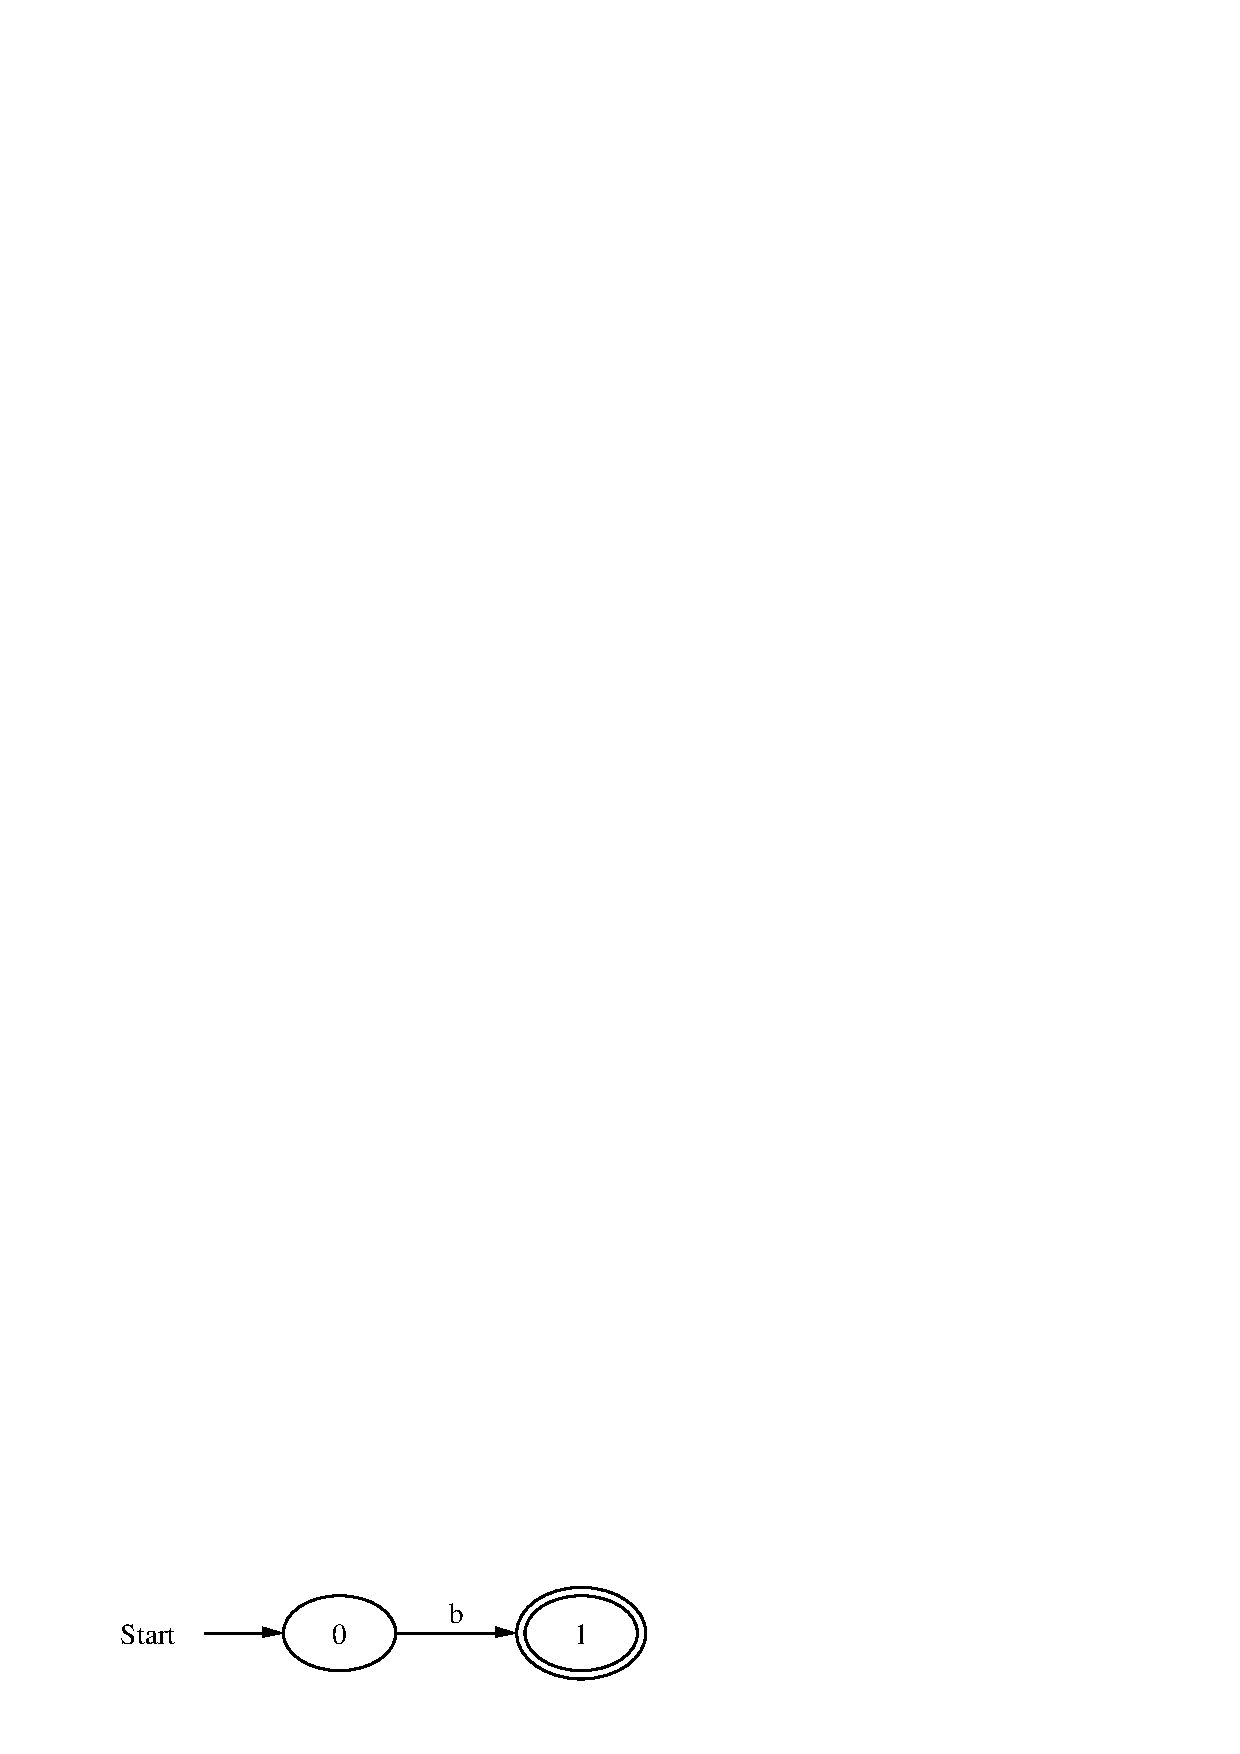
\epsfig{file=lettera}

\begin{enumerate}
\item 2 Zust"ande
\item $0 \stackrel{b}{\rightarrow} 1$
\item $1 \stackrel{\varepsilon}{\rightarrow} 1$
\end{enumerate}

Implementierung:
\begin{verbatim}
FSM* createCharacter(char c) {
    FSM* fsm = allocateFSM(2);
    charTransition(fsm, 0, 1, c);
    epsTransition (fsm, 1, 1, 1);
    return fsm;
}
\end{verbatim}

\vspace*{\fill}
\tiny \addtocounter{mypage}{1}
\rule{17cm}{1mm}
Pattern Matching \hspace*{\fill} Seite \arabic{mypage}
\end{slide}

%%%%%%%%%%%%%%%%%%%%%%%%%%%%%%%%%%%%%%%%%%%%%%%%%%%%%%%%%%%%%%%%%%%%%%%%%

\begin{slide}{}
\normalsize

\begin{center}
Implementierung der Konkatenation
\end{center}
\vspace*{0.5cm}

\footnotesize
\hspace*{1.3cm} \raisebox{1cm}{Start $\rightarrow$}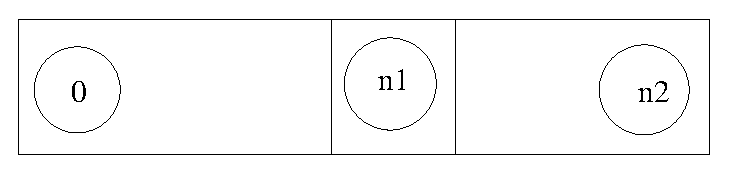
\epsfig{file=append.eps}

Implementierung
\begin{enumerate}
\item Gr"o\3e Fsm \texttt{f1}: \texttt{n1}.
\item Gr"o\3e Fsm \texttt{f2}: \texttt{n2}.
\item Gr"o\3e neue Fsm: \texttt{n1 + n2 - 1}
\item Kopiere \texttt{f1} an Offsett 0 in neuer Fsm.
\item Kopiere \texttt{f2} an Offsett \texttt{n1-1} in neuer Fsm.
\end{enumerate}
\vspace*{0.5cm}

\begin{verbatim}
    FSM* concat(FSM* f1, FSM* f2) {
        unsigned n1 = f1 ->numberStates;
        unsigned n2 = f2 ->numberStates;
        unsigned n  = n1 + n2 - 1;
        FSM* fsm = allocateFSM(n);
        move(fsm, f1, 0);
        move(fsm, f2, n1 - 1);
        freeFsm(f1);
        freeFsm(f2);
        return fsm;
    }
\end{verbatim}

\vspace*{\fill}
\tiny \addtocounter{mypage}{1}
\rule{17cm}{1mm}
Pattern Matching \hspace*{\fill} Seite \arabic{mypage}
\end{slide}

%%%%%%%%%%%%%%%%%%%%%%%%%%%%%%%%%%%%%%%%%%%%%%%%%%%%%%%%%%%%%%%%%%%%%%%%%

\begin{slide}{}
\normalsize

\begin{center}
Implementierung der Alternative
\end{center}
\vspace*{0.5cm}

\footnotesize
\hspace*{-1cm}
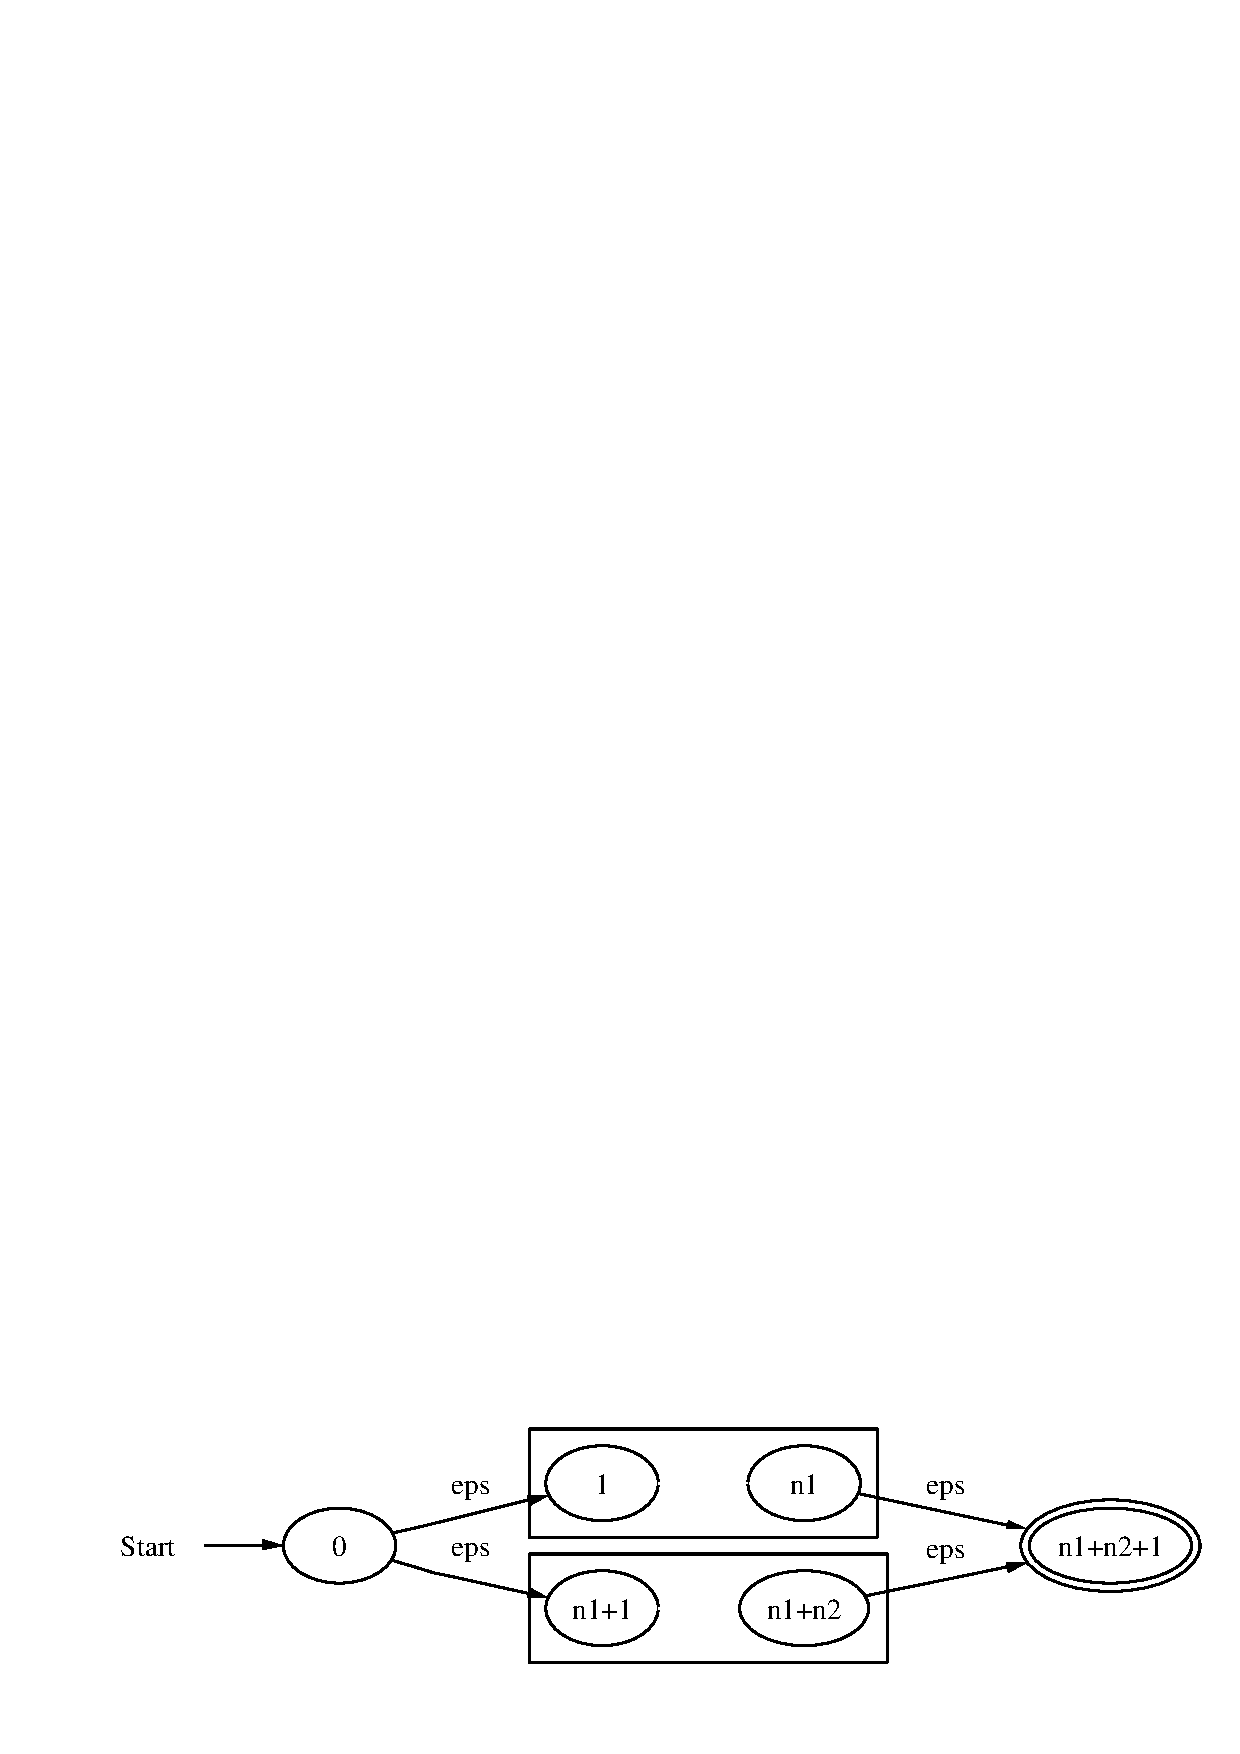
\epsfig{file=alternationa}

Implementierung
\begin{enumerate}
\item Gr"o\3e Fsm \texttt{f1}: \texttt{n1}.
\item Gr"o\3e Fsm \texttt{f2}: \texttt{n2}.
\item Gr"o\3e neue Fsm: \texttt{n1 + n2 + 2}
\item Kopiere \texttt{f1} an Offsett 1 in neuer Fsm.
\item Kopiere \texttt{f2} an Offsett \texttt{n1+1} in neuer Fsm.
\end{enumerate}

\begin{verbatim}
    FSM* alternative(FSM* f1, FSM* f2) {
        unsigned n1 = f1 ->numberStates;
        unsigned n2 = f2 ->numberStates;
        unsigned n  = n1 + n2 + 2;
        FSM* fsm = allocateFSM(n);
        epsTransition(fsm, 0, 1, n1 + 1);
        move(fsm, f1, 1);
        move(fsm, f2, n1 + 1);
        epsTransition(fsm, n1, n - 1, n - 1);
        epsTransition(fsm, n - 2, n - 1, n - 1);
        epsTransition(fsm, n - 1, n - 1, n - 1);
        freeFsm(f1);   freeFsm(f2);
        return fsm;
    }
\end{verbatim}


\vspace*{\fill}
\tiny \addtocounter{mypage}{1}
\rule{17cm}{1mm}
Pattern Matching \hspace*{\fill} Seite \arabic{mypage}
\end{slide}

%%%%%%%%%%%%%%%%%%%%%%%%%%%%%%%%%%%%%%%%%%%%%%%%%%%%%%%%%%%%%%%%%%%%%%%%%

\begin{slide}{}
\normalsize

\begin{center}
Implementierung des Abschlusses
\end{center}
\vspace*{0.5cm}

\footnotesize
\hspace*{-1cm}
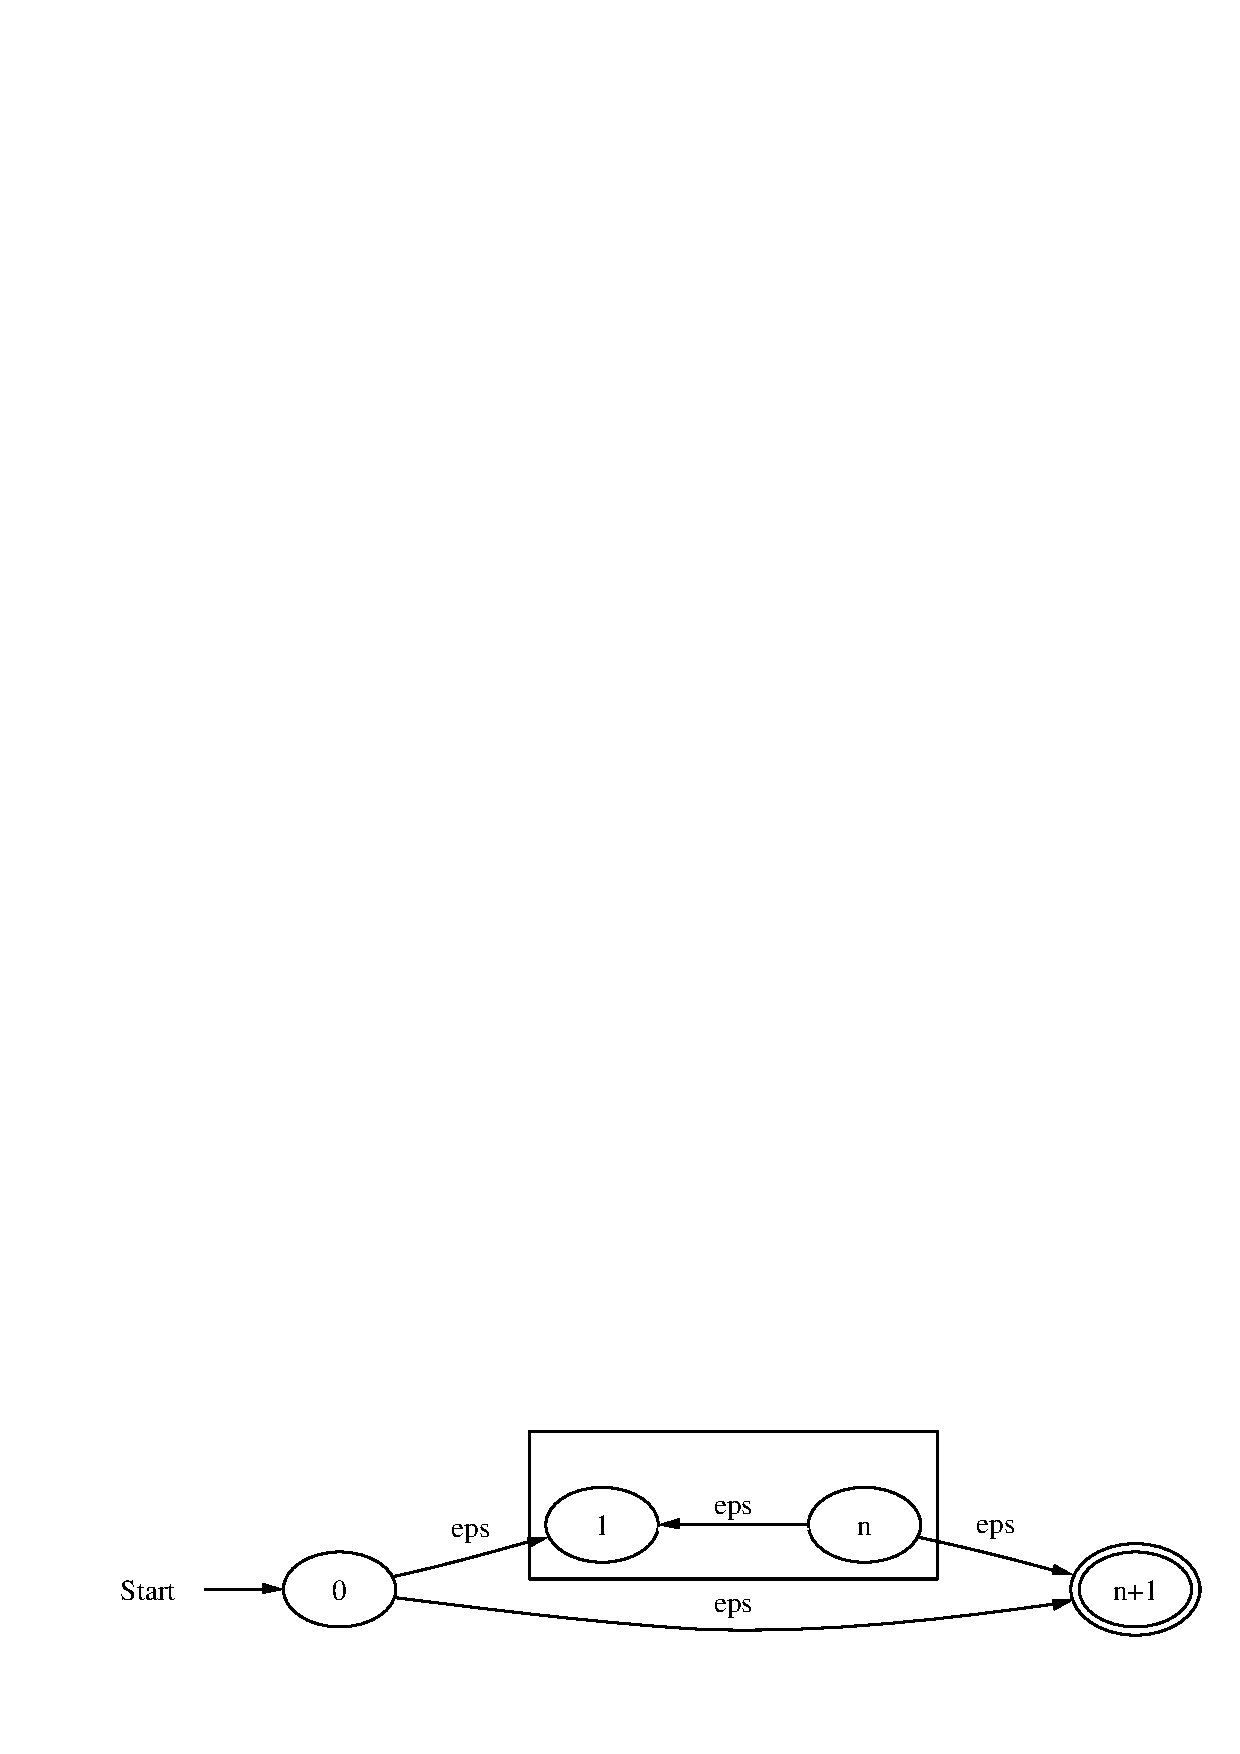
\epsfig{file=closurea}

\begin{enumerate}
\item Gr"o\3e Fsm \texttt{f}: \texttt{n}.
\item Gr"o\3e neue Fsm: \texttt{n + 2}
\item Kopiere \texttt{f} an Offsett 1 in neuer Fsm.
\end{enumerate}

Implementierung
\begin{verbatim}
    FSM* closure(FSM* f) {
        unsigned n = f->numberStates;
        FSM* fsm = allocateFSM(n+2);
        epsTransition(fsm, 0, 1, n + 1);
        move(fsm, f, 1);
        epsTransition(fsm, n, n + 1, 1);
        epsTransition(fsm, n + 1, n + 1, n + 1);
        freeFsm(f);
        return fsm;
    }
\end{verbatim}


\vspace*{\fill}
\tiny \addtocounter{mypage}{1}
\rule{17cm}{1mm}
Pattern Matching \hspace*{\fill} Seite \arabic{mypage}
\end{slide}

%%%%%%%%%%%%%%%%%%%%%%%%%%%%%%%%%%%%%%%%%%%%%%%%%%%%%%%%%%%%%%%%%%%%%%%%%

\begin{slide}{}
\normalsize

\begin{center}
Konstruktion einer \texttt{RegExp} aus einer FSM
\end{center}
\vspace*{0.5cm}

\footnotesize
\textbf{Definitionen}: Sei $\Sigma$ ein endliches Alphabet.
\begin{enumerate}
\item  Es seien $\Ll_1, \Ll_2 \subseteq \Sigma^*$. Wir definieren die\\ 
       \emph{Konkatenation} von $\Ll_1$ und $\Ll_2$ als:\\[0.3cm]
      \hspace*{1.3cm} $\Ll_1 \Ll_2 := \bigg\{ vw  \;|\; v \in \Ll_1 \wedge w \in \Ll_2 \}$
\item Sei $\Ll \subseteq \Sigma^*$. F"ur $n \in \mathbb{N}$ definieren wir die \emph{Potenz} $\Ll^n$ durch
      Induktion "uber $n$:
      \begin{enumerate}
      \item[I.A.] $n \mapsto 0$:    \hspace*{2.3cm} $\Ll^0 := \{ \varepsilon \}$
      \item[I.S.] $n \mapsto n+1$: \hspace*{1.0cm} $\Ll^{n+1} := \Ll^n \Ll$
      \end{enumerate}
\item Sei $\Ll \subseteq \Sigma^*$. Wir definieren den \emph{Abschlu\3} von $\Ll$ als \\[0.3cm]
      \hspace*{1.3cm} $\Ll^* = \bigcup\limits_{n=0}^\infty \Ll^n$
\item Seien $u,w \in \Sigma^*$.  $u$ ist \emph{Pr"afix} von $w$,
      g.d.w. es gibt $v \in \Sigma^*$  mit $v \not= \varepsilon$ und $uv = w$.
      Schreibweise: $u \prec w$        \\[0.3cm]
      \hspace*{1.3cm} $u \prec w \;\Leftrightarrow\; \exists v \in \Sigma^*: v \not= \varepsilon \wedge uv = w$.
\end{enumerate}
\textbf{Beispiele}: Sei $\Sigma = \{a,b\}$, $\Ll_1 = \{ba, b\}$ und $\Ll_2 = \{abb, bb\}$.
\begin{enumerate}
\item $\Ll_1\Ll_2 = \{ baabb, babb, babb, bbb\}$
\item $\Ll_1^3 = \{ bbb, bbba, bbab, babb, babab, babba, bbaba, bababa \}$
\item $abbabb \prec abbabbabb$
\end{enumerate}

\vspace*{\fill}
\tiny \addtocounter{mypage}{1}
\rule{17cm}{1mm}
Pattern Matching \hspace*{\fill} Seite \arabic{mypage}
\end{slide}

%%%%%%%%%%%%%%%%%%%%%%%%%%%%%%%%%%%%%%%%%%%%%%%%%%%%%%%%%%%%%%%%%%%%%%%%%

\begin{slide}{}
\normalsize

\begin{center}
Weitere Definitionen
\end{center}
\vspace*{0.5cm}

\footnotesize
\textbf{Definition}: Gegeben sei eine FSM \\[0.3cm]
\hspace*{1.3cm} $F = \langle \Sigma, \{q_1,\cdots,q_n\}, A, q_1, \mathtt{next}  \rangle$ 

Wir definieren eine partielle Funktion \\[0.3cm]
\hspace*{1.3cm} $\mathtt{next}^{(k)}: Z \times \Sigma^* \rightarrow Z$
\begin{enumerate}
\item Fall: $\forall v \in \Sigma^*\backslash \{\varepsilon\}: v \prec w \rightarrow \mathtt{next}(q,v) \in \{q_1,\cdots,q_k\}$

      Dann setzen wir \\[0.3cm]
      \hspace*{1.3cm} $\mathtt{next}^{(k)}(q, w) = \mathtt{next}^*(q,w)$.
\item Fall: $\exists v \in \Sigma^*\backslash \{\varepsilon\}:  v \prec w \wedge \mathtt{next}(q,v) \not\in \{q_1,\cdots,q_k\}$

      Dann sei $\mathtt{next}^{(k)}(q, w)$ undefiniert, wir setzen \\[0.3cm]
      \hspace*{1.3cm} $\mathtt{next}^{(k)}(q, w) =\; \uparrow$.
\end{enumerate}
Falls $\mathtt{next}^{(k)}(q,w) = p$ ist, so sagen wir, dass die Berechnung
von $w$ im Zustand $q$, die Zust"ande aus $\{q_{k+1}, \cdots, q_n\}$ \emph{vermeidet}.

F"ur $k \in \{0,1,\cdots,n\}$ und $i,j\in \{1,\cdots,n\}$ 
definieren wir Sprachen $\Rl_{i,j}^{(k)}$ \\[0.3cm]
\hspace*{1.3cm} $\Rl_{i,j}^{(k)} := \bigg\{ w \in \Sigma^* \;|\; \mathtt{next}^{(k)}(q_i,w) = q_j \bigg\}$

\textbf{Bemerkung}: Es gilt \\[0.3cm]
\hspace*{1.3cm} $\Rl_{i,j}^{(n)} := \bigg\{ w \in \Sigma^* \;|\; \mathtt{next}^*(q_i,w) = q_j \bigg\}$

\vspace*{\fill}
\tiny \addtocounter{mypage}{1}
\rule{17cm}{1mm}
Pattern Matching \hspace*{\fill} Seite \arabic{mypage}
\end{slide}

%%%%%%%%%%%%%%%%%%%%%%%%%%%%%%%%%%%%%%%%%%%%%%%%%%%%%%%%%%%%%%%%%%%%%%%%

\begin{slide}{}
\normalsize

\begin{center}
Konstruktion einer \texttt{RegExp} aus einer FSM 
\end{center}

\footnotesize
\textbf{Gegeben}: FSM $F = \langle \Sigma, \{q_1,\cdots,q_n\}, A, q_1, \mathtt{next} \rangle$

\textbf{Gesucht}: $r \in \mathtt{RegExp}$ mit $\Ll(r) = \Ll(F)$

Wir geben induktive Konstruktionen der  Sprachen
 $\Rl_{i,j}^{(k)}$: 
\begin{enumerate}
\item Induktions--Anfang: $k=0$
  \begin{enumerate}
  \item $\exists a \in \Sigma:\mathtt{next}(q_i, a) = q_j$ und $i\not=j$\\[0.3cm]
        \hspace*{1.3cm} $\Rl_{i,j}^{(0)} := \{a\}$
  \item $\exists a \in \Sigma:\mathtt{next}(q_i, a) = q_i$ \\[0.3cm]
        \hspace*{1.3cm} $\Rl_{i,i}^{(0)} := \{a,\varepsilon\}$
  \item $\forall a \in \Sigma:\mathtt{next}(q_i, a) \not= q_j$ und $i\not=j$ \\[0.3cm]
        \hspace*{1.3cm} $\Rl_{i,j}^{(0)} := \{\}$
  \item $\forall a \in \Sigma:\mathtt{next}(q_i, a) \not= q_i$ und $i=j$ \\[0.3cm]
        \hspace*{1.3cm} $\Rl_{i,i}^{(0)} := \{\varepsilon\}$
  \end{enumerate}
\item Induktions--Schritt: $k \mapsto k + 1$ 

     \hspace*{1.3cm} $\Rl_{i,j}^{(k+1)} := \Rl_{i,j}^{(k)} \cup \Rl_{i,k+1}^{(k)} \left(\Rl_{k+1,k+1}^{(k)}\right)^* \Rl_{k+1,j}^{(k)}$     \\[0.5cm]
     Begr"undung: Es ist $w \in \Rl_{i,j}^{(k+1)}$ g.d.w. 
     \begin{enumerate}
     \item $w \in \Rl_{i,j}^{(k)}$ oder
     \item $w =x v_1v_2 \cdots v_n y$ mit $n\geq 0$ und
       \begin{itemize}
       \item $x \in \Rl_{i,k+1}^{(k)}$, \quad $y \in \Rl_{k+1,j}^{(k)}$

       \item $v_i \in \Rl_{k+1,k+1}^{(k)}$ f"ur alle $i=1,\cdots,n$
       \end{itemize}
     \end{enumerate}
\end{enumerate}


\vspace*{\fill}
\tiny \addtocounter{mypage}{1}
\rule{17cm}{1mm}
Pattern Matching \hspace*{\fill} Seite \arabic{mypage}
\end{slide}

%%%%%%%%%%%%%%%%%%%%%%%%%%%%%%%%%%%%%%%%%%%%%%%%%%%%%%%%%%%%%%%%%%%%%%

\begin{slide}{}
\normalsize

\begin{center}
  Abschlu\3 der Konstruktion
\end{center}

\footnotesize
Wir definieren regul"are Ausdr"ucke $r_{i,j}^{(k)}$ mit \\[0.3cm]
\hspace*{1.3cm} $\Ll(r_{i,j}^{(k)}) = \Rl_{i,j}^{(k)}$

\begin{enumerate}
\item Induktions--Anfang: $k=0$
  \begin{enumerate}
  \item $\exists a \in \Sigma:\mathtt{next}(q_i, a) = q_j$ und $i \not= j$ \\[0.3cm]
        \hspace*{1.3cm} $r_{i,j}^{(0)} := a$
  \item $\exists a \in \Sigma:\mathtt{next}(q_i, a) = q_i$  \\[0.3cm]
        \hspace*{1.3cm} $r_{i,i}^{(0)} := a + \varepsilon$
  \item $\forall a \in \Sigma:\mathtt{next}(q_i, a) \not= q_j$ und $i\not=j$ \\[0.3cm]
        \hspace*{1.3cm} $r_{i,j}^{(0)} := \emptyset$
  \item $\forall a \in \Sigma:\mathtt{next}(q_i, a) \not= q_i$ \\[0.3cm]
        \hspace*{1.3cm} $r_{i,i}^{(0)} := \varepsilon$
  \end{enumerate}
\item Induktions--Schritt: $k \mapsto k + 1$ 

      \hspace*{1.3cm} $r_{i,j}^{(k+1)} := r_{i,j}^{(k)} + r_{i,k+1}^{(k)} \left(r_{k+1,k+1}^{(k)}\right)^* r_{k+1,j}^{(k)}$ 
\end{enumerate}
Setze  $r_{i,j} := r_{i,j}^{(n)}$.

Sei $A = \{q_l, \cdots, q_n\}$ Menge der akzeptierenden Zust"ande. \\[0.3cm]
\hspace*{1.3cm}  $r_F := r_{1,l} + r_{1,l+1} + \cdots + r_{1,n}$. \\[0.3cm]
 Dann gilt \\[0.3cm]
\hspace*{1.3cm} $\Ll(F) = \Ll\bigg(r_F\bigg)$ 

\vspace*{\fill}
\tiny \addtocounter{mypage}{1}
\rule{17cm}{1mm}
Pattern Matching \hspace*{\fill} Seite \arabic{mypage}
\end{slide}

%%%%%%%%%%%%%%%%%%%%%%%%%%%%%%%%%%%%%%%%%%%%%%%%%%%%%%%%%%%%%%%%%%%%%%%%%

\begin{slide}{}
\normalsize

\begin{center}
Ein Beispiel 
\end{center}
\vspace*{0.5cm}

\footnotesize
\textbf{Definition}: Eine deterministische FSM \\[0.3cm]
\hspace*{1.3cm} $F = \langle \Sigma, Z, A, s_0, \mathtt{next}  \rangle$  \\[0.3cm]
ist eine \emph{partielle} FSM, wenn die Funktion \texttt{next} teilweise undefiniert ist.

\textbf{Bemerkung}: Die Konstruktion eines regul"aren Ausdrucks $r$ mit \\[0.3cm]
\hspace*{1.3cm} $\Ll(r) = \Ll(F)$ \\[0.3cm]
funktioniert auch f"ur partielle FSMs.
\vspace*{0.5cm}

\textbf{Aufgabe}: Berechnen Sie f"ur folgende FSM einen "aquivalenten regul"aren Ausdruck. \\[0.6cm]
\hspace*{1.3cm} 
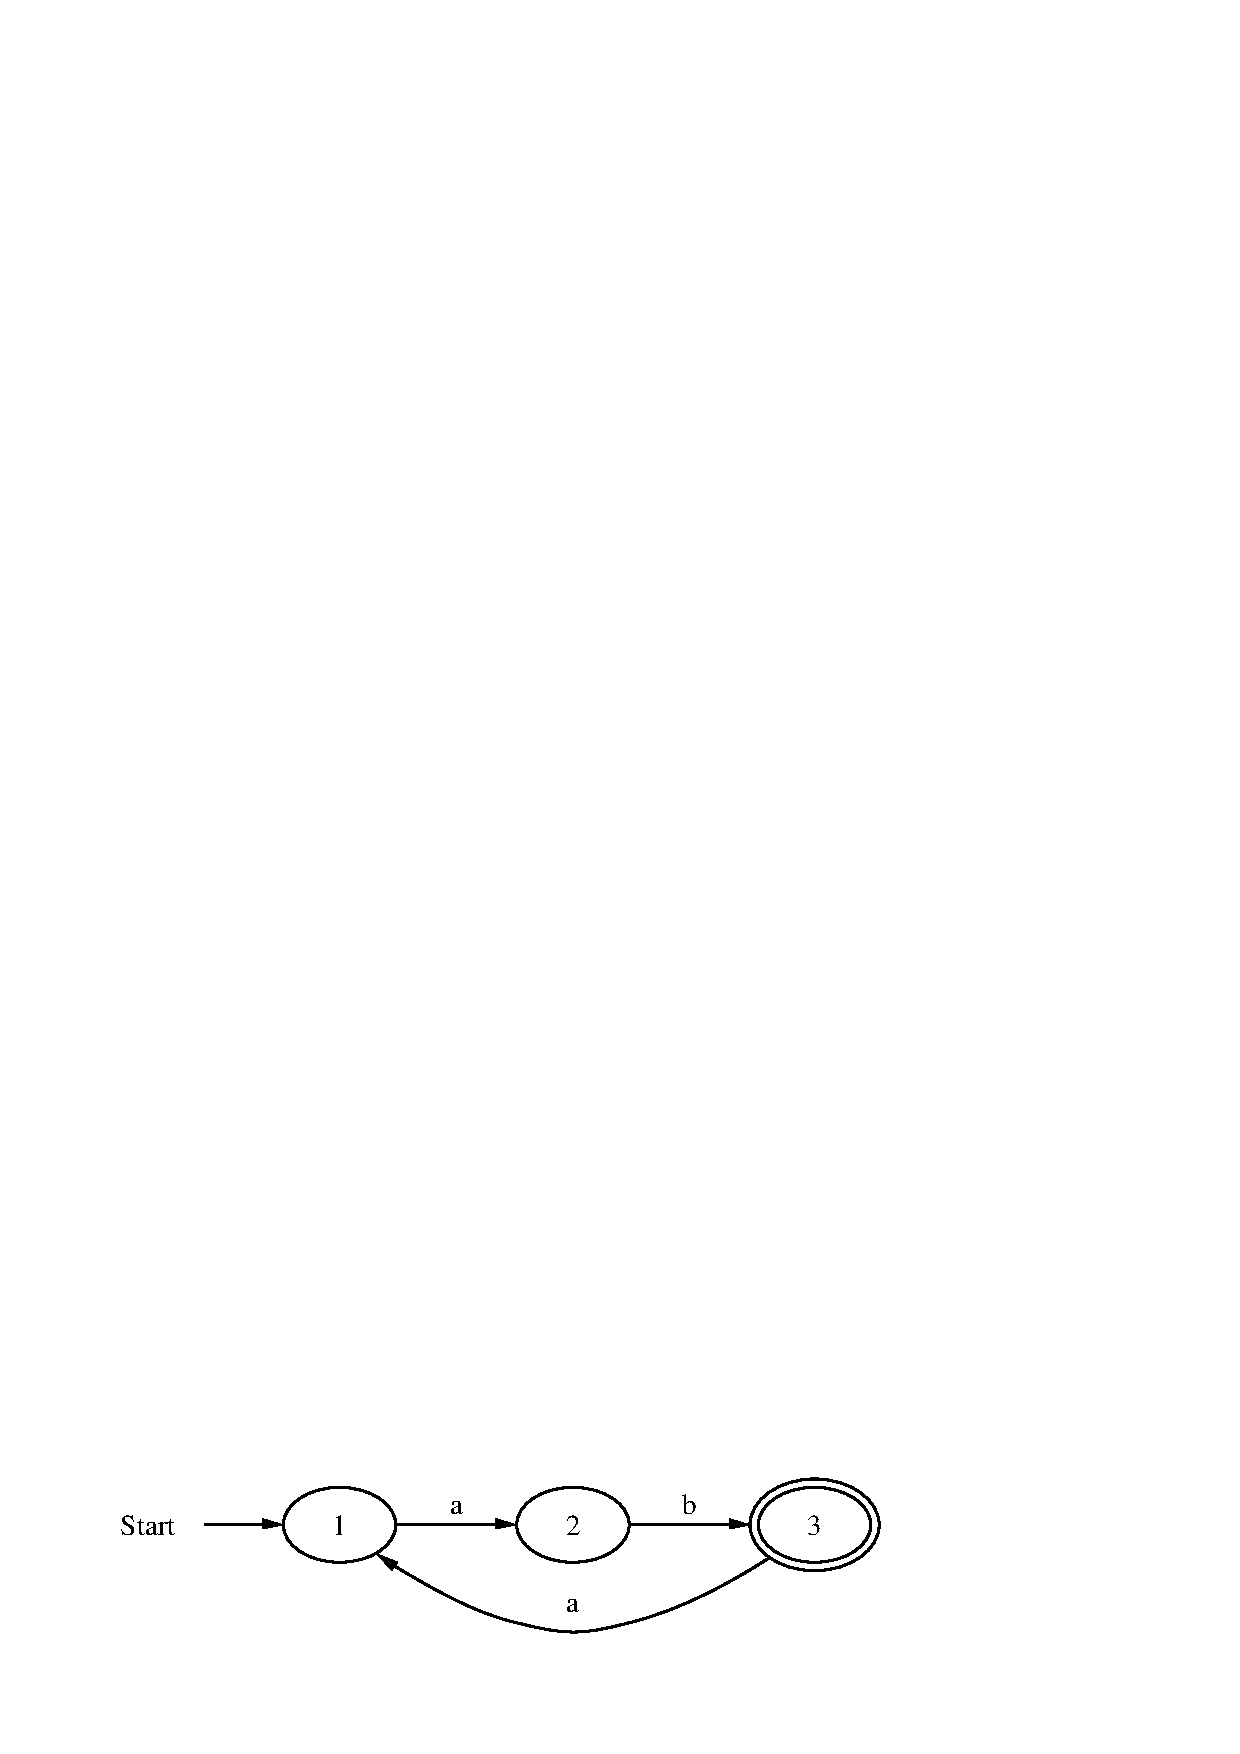
\epsfig{file=partial}

N"utzliche Vereinfachungs--Regeln
\begin{enumerate}
\item $(\varepsilon + r)^* \simeq r*$
\item $(\varepsilon + r) (\varepsilon + r)^* \simeq r^*$
\item $r_1 + r_1 r_2^* \simeq r_1 r_2^*$
\item $r_1 + r_1 r_2 r_2^* \simeq r_1 r_2^*$
\item $r_1(r_2r_1)^*r_2 = r_1r_2(r_1r_2)^*$
\end{enumerate}

\vspace*{\fill}
\tiny \addtocounter{mypage}{1}
\rule{17cm}{1mm}
Pattern Matching \hspace*{\fill} Seite \arabic{mypage}
\end{slide}

%%%%%%%%%%%%%%%%%%%%%%%%%%%%%%%%%%%%%%%%%%%%%%%%%%%%%%%%%%%%%%%%%%%%%%%%%

\begin{slide}{}
\normalsize

\begin{center}
Berechnung des regul"aren Ausdrucks
\end{center}

\footnotesize
\hspace*{1.3cm}
\begin{tabular}{|l|l|l|l|l|}
\hline
                & $k = 0$ & $k = 1$ & $k = 2$ & $k = 3$ \\
\hline
\hline
$r_{1,1}^{(k)}$ & $\varepsilon$ & $\varepsilon$ & $\varepsilon$ & $(aba)^*$ \\
\hline
$r_{1,2}^{(k)}$ & $a$ & $a$ & $a$ & $a(baa)^*$ \\
\hline
$r_{1,3}^{(k)}$ & $\emptyset$ & $\emptyset$ & $ab$ & $ab(aab)^*$ \\
\hline
$r_{2,1}^{(k)}$ & $\emptyset$ & $\emptyset$  & $\emptyset$ & $ba(aba)^*$ \\
\hline
$r_{2,2}^{(k)}$ & $\varepsilon$ & $\varepsilon$ & $\varepsilon$ & $(baa)^*$ \\
\hline
$r_{2,3}^{(k)}$ & $b$ & $b$ & $b$ & $b(baa)^*$ \\
\hline
$r_{3,1}^{(k)}$ & $a$ & $a$ & $a$ & $a(aba)^*$ \\
\hline
$r_{3,2}^{(k)}$ & $\emptyset$ & $aa$ & $aa$ & $aa(baa)^*$ \\
\hline
$r_{3,3}^{(k)}$ & $\varepsilon$ & $\varepsilon$ & $\varepsilon + aab$ & $(aab)^*$ \\
\hline
\end{tabular}

\begin{enumerate}
\item Spalte: folgt unmittelbar aus Diagramm
      \vspace*{-0.5cm}
\item Spalte: einzige "Anderung dort, wo Pfade der L"ange 2 sind, deren mittlerer Knoten 1 ist: \\[0.3cm]
      \hspace*{1.3cm} $3 \stackrel{a}{\rightarrow} 1 \stackrel{a}{\rightarrow} 2$, also $r_{3,2}^{(1)} = aa$
      \vspace*{-0.5cm}
\item Spalte: einzige "Anderung dort, wo Pfade mit Knoten 2 hinzukommen: \\[0.3cm]
      \hspace*{1.3cm} $3 \stackrel{a}{\rightarrow} 1 \stackrel{a}{\rightarrow} 2 \stackrel{b}{\rightarrow} 3$, also $r^{(2)}_{3,3} = \varepsilon + aab$ \\[0.3cm]
      \hspace*{1.3cm} $1 \stackrel{a}{\rightarrow} 2 \stackrel{b}{\rightarrow} 3$, also $r_{1,3}^{(2)} = ab$
      \vspace*{-0.5cm}
\item Spalte: Sei $i \stackrel{u}{\rightarrow} j$ und $j \stackrel{v}{\rightarrow} j$ \\[0.3cm]
      \hspace*{1.3cm} $r_{i,j}^{(3)} = uv^*$ 
\end{enumerate}
Also: \quad $\Ll(F) = \Ll\bigg(ab(aab)^*\bigg)$

\vspace*{\fill}
\tiny \addtocounter{mypage}{1}
\rule{17cm}{1mm}
Pattern Matching \hspace*{\fill} Seite \arabic{mypage}
\end{slide}

%%%%%%%%%%%%%%%%%%%%%%%%%%%%%%%%%%%%%%%%%%%%%%%%%%%%%%%%%%%%%%%%%%%%%%%%%

\begin{slide}{}
\normalsize

\begin{center}
Pumping Lemma
\end{center}
\vspace*{0.5cm}

\footnotesize
\textbf{Definition}: F"ur ein Wort $w \in \Sigma^*$ bezeichnet \\[0.3cm]
\hspace*{1.3cm} $|w|$ \\[0.3cm]
die \emph{L"ange} (Zahl der Buchstaben) von $w$.

F"ur $n \in \mathbb{N}$ definieren wir $w^n$ induktiv:
\begin{enumerate}
\item[I.A.] $n \mapsto 0$:   \hspace*{2.5cm} $w^0 := \varepsilon$
\item[I.S.] $n \mapsto n+1$: \hspace*{1.3cm} $w^{n+1} := w w^n$

\end{enumerate}

\textbf{Definition}: Sei $\Sigma$ Alphabet. Eine Sprache $\Ll \subseteq \Sigma^*$
ist \emph{regul"ar der Ordnung $n$} g.d.w. es einen endl. Automaten \\[0.3cm]
\hspace*{1.3cm} $F = \langle \Sigma, Z, A, s_0, \mathtt{next} \rangle$ \\[0.3cm]
gibt, so da\3 gilt: \quad $\Ll = \Ll(F)$ und $\mathtt{card}(Z) = n$.

Hier bezeichnet $\texttt{card}(Z)$ die Zahl der Zust"ande.

\textbf{Satz} (\textsl{Pumping Lemma}) \\[0.3cm]
\textbf{Vor.}: $\Ll$ ist regul"are Sprache der Ordnung $n$.

\textbf{Beh.}: F"ur alle $w \in \Ll$ mit $|w| \geq n$ gibt es $x,y,z \in \Sigma^*$ mit
\begin{enumerate}
\item $w = xyz$
\item $|xy| \leq n$
\item $|y| \geq 1$
\item $\forall k \in \mathbb{N}: x y^k z \in \Sigma^*$
\end{enumerate}

\vspace*{\fill}
\tiny \addtocounter{mypage}{1}
\rule{17cm}{1mm}
Pattern Matching \hspace*{\fill} Seite \arabic{mypage}
\end{slide}

%%%%%%%%%%%%%%%%%%%%%%%%%%%%%%%%%%%%%%%%%%%%%%%%%%%%%%%%%%%%%%%%%%%%%%%%%

\begin{slide}{}
\normalsize

\begin{center}
Beweis des Pumping Lemma
\end{center}

\footnotesize
Sei $\Ll = \Ll(F)$ mit \quad  $F = \langle \Sigma, Z, q_0, \mathtt{next} \rangle$ und $n = \mathtt{card}(Z)$.

Sei $w = a_1a_2 \cdots a_m \in \Ll(F)$ mit $m \geq n$.  Dann gibt es Berechnung der FSM $F$ mit Label $w$:
\\[0.3cm]
\hspace*{1.3cm} 
  $q_0 \stackrel{a_1}{\rightarrow} q_1 \stackrel{a_2}{\rightarrow} q_2 \stackrel{a_3}{\rightarrow} \cdots \stackrel{a_m}{\rightarrow} q_m$ \quad und $q_m \in A$ 
  \\[0.3cm]
Es k"onnen nicht alle Zust"ande in der Menge \\[0.3cm]
\hspace*{1.3cm} $\{q_0, q_1, q_2, \cdots, q_n\}$ \\[0.3cm]
verschieden sein, es gibt also $i,j \in \{0,\cdots,n\}$ mit \\[0.3cm]
\hspace*{1.3cm} $i < j$ \quad und \quad $q_i = q_j$. \\[0.3cm]
Wir definieren \\[0.3cm]
\hspace*{1.3cm} $x := a_1 \cdots a_i$, \quad $y := a_{i+1} \cdots a_j$, \quad 
                $z := a_{j+1} \cdots a_m$ \\[0.3cm]
Dann haben wir die folgenden Berechnungen der FSM $F$ \\[0.3cm]
\hspace*{1.3cm} 1. $q_0 \stackrel{a_1}{\rightarrow} \cdots \stackrel{a_i}{\rightarrow} q_i$, also $q_0 \stackrel{x}{\rightarrow} q_i$ \\[0.3cm] 
\hspace*{1.3cm} 2. $q_i \stackrel{a_{i+1}}{\rightarrow} \cdots \stackrel{a_j}{\rightarrow} q_i$, also $q_i \stackrel{y}{\rightarrow} q_i$ \\[0.3cm] 
\hspace*{1.3cm} 3. $q_i \stackrel{a_{j+1}}{\rightarrow} \cdots \stackrel{a_m}{\rightarrow} q_m$, also $q_i \stackrel{z}{\rightarrow} q_m$ \\[0.3cm] 
Damit gilt auch \\[0.3cm]
\hspace*{1.3cm} $q_0 \stackrel{x}{\rightarrow} \underbrace{q_i \stackrel{y}{\rightarrow} q_i \stackrel{y}{\rightarrow} \cdots \stackrel{y}{\rightarrow} q_i}_{k}
\stackrel{z}{\rightarrow} q_m$ \\[0.3cm]
und das zeigt, dass \\[0.3cm]
\hspace*{1.3cm} $x y^k z \in \Ll$ \quad f"ur alle $k \in \mathbb{N}$ \\[0.3cm]
Aus $i < j$ und  $|y| = j - i$ folgt $|y| \geq 1$. \\[0.3cm]
Wegen $|xy| = j$ und $j \in \{0,\cdots,n\}$ folgt auch \\[0.3cm]
\hspace*{1.3cm} $|xy| \leq n$. \hspace*{\fill} $\Box$

\vspace*{\fill}
\tiny \addtocounter{mypage}{1}
\rule{17cm}{1mm}
Pattern Matching \hspace*{\fill} Seite \arabic{mypage}
\end{slide}

%%%%%%%%%%%%%%%%%%%%%%%%%%%%%%%%%%%%%%%%%%%%%%%%%%%%%%%%%%%%%%%%%%%%%%%%%

\begin{slide}{}
\normalsize

\begin{center}
Anwendung des Pumping Lemma
\end{center}
\vspace*{0.5cm}

\footnotesize
\textbf{Aufgabe}: Sei $\Sigma = \{\mathtt{a},\mathtt{b}\}$. Zeigen Sie, dass die Sprache \\[0.3cm]
\hspace*{1.3cm}  $\Ll := \bigg\{ w \in \Sigma^* \;|\; \mathtt{nr}(w,\mathtt{a}) = \mathtt{nr}(w,\mathtt{b}) \bigg\}$ \\[0.3cm]
nicht regul"ar ist. 

Ein Wort in $\Ll$ enth"alt genauso viele Buchstaben \texttt{a} wie \texttt{b}.

\textbf{Beweis} indirekt. \\[0.3cm]
\textbf{Annahme}: Sei $\Ll$ regul"are Sprache der Ordnung $n$.  \\
Betrachte das Wort $w := a^nb^n$.   Es gilt \\[0.3cm]
\hspace*{1.3cm} $a^nb^n \in \Ll$ \quad und \quad $|a^nb^n| = 2*n$. \\[0.3cm]
Also gibt es  Worte $x$, $y$ und $z$ mit:
\begin{enumerate}
\item $w = a^nb^n = xyz$
\item $|xy| \leq n$
\item $|y| \geq 1$
\item $xy^kz \in \Ll$
\end{enumerate}
Aus \quad $|xy| \leq n$ \quad und \quad $xyz = a^nb^n$ \quad folgt \\[0.3cm]
\hspace*{1.3cm}  $xy \prec a^n$ \\[0.3cm]
und daraus folgt \\[0.3cm]
\hspace*{1.3cm} $\mathtt{nr}(x, \mathtt{b}) = 0$ \quad und \quad $\mathtt{nr}(y, \mathtt{b}) = 0$. \\[0.3cm]

\vspace*{\fill}
\tiny \addtocounter{mypage}{1}
\rule{17cm}{1mm}
Pattern Matching \hspace*{\fill} Seite \arabic{mypage}
\end{slide}

%%%%%%%%%%%%%%%%%%%%%%%%%%%%%%%%%%%%%%%%%%%%%%%%%%%%%%%%%%%%%%%%%%%%%%%%%

\begin{slide}{}
\normalsize

\begin{center}
Fortsetzung der Aufgabe
\end{center}
\vspace*{0.5cm}

\footnotesize
Aus $xyz \in \Ll$ folgt wegen \\[0.3cm]
\hspace*{1.3cm} $\mathtt{nr}(xyz, \mathtt{a}) = \mathtt{nr}(x,\mathtt{a)} + \mathtt{nr}(y,\mathtt{a)} + \mathtt{nr}(z,\mathtt{a)}$  und \\[0.3cm]
\hspace*{1.3cm}
 $\mathtt{nr}(xyz, \mathtt{b}) = \mathtt{nr}(x,\mathtt{b)} + \mathtt{nr}(y,\mathtt{b)} + \mathtt{nr}(z,\mathtt{b)} = \mathtt{nr}(z,b)$ \\[0.3cm]
die Gleichung \\[0.3cm]
\hspace*{1.3cm}  $\mathtt{nr}(x,\mathtt{a)} + \mathtt{nr}(y,\mathtt{a)} + \mathtt{nr}(z,\mathtt{a)} =  \mathtt{nr}(z,b)$ \hspace*{\fill} (A) \\[0.3cm]
Ebenso folgt aus $xy^2z \in \Ll$ und \\[0.3cm]
\hspace*{1.3cm} $\mathtt{nr}(xy^2z, \mathtt{a}) = \mathtt{nr}(x,\mathtt{a)} + 2 * \mathtt{nr}(y,\mathtt{a)} + \mathtt{nr}(z,\mathtt{a)}$  und \\[0.3cm]
\hspace*{1.3cm} $\mathtt{nr}(xy^2z, \mathtt{b}) = \mathtt{nr}(x,\mathtt{b)} + 2 * \mathtt{nr}(y,\mathtt{b)} + \mathtt{nr}(z,\mathtt{b)} = \mathtt{nr}(z,b)$ \\[0.3cm]
die Gleichung \\[0.3cm]
\hspace*{1.3cm}  $\mathtt{nr}(x,\mathtt{a)} + 2 *\mathtt{nr}(y,\mathtt{a)} + \mathtt{nr}(z,\mathtt{a)} =  \mathtt{nr}(z,b)$ \hspace*{\fill} (B) \\[0.3cm]
Ziehen wir (A) von (B) ab, so erhalten wir \\[0.3cm]
\hspace*{1.3cm} $\mathtt{nr}(y,a) = 0$ \\[0.3cm]
Weil auch \\[0.3cm]
\hspace*{1.3cm} $\mathtt{nr}(y,b) = 0$ \\[0.3cm]
gilt, folgt \\[0.3cm]
\hspace*{1.3cm} $y = \varepsilon$ \\[0.3cm]
Das steht im Widerspruch zu\\[0.3cm]
\hspace*{1.3cm}  $|y| \geq 1$ . \hspace*{\fill} $\Box$

\textbf{Erkenntnis}: Endliche Automaten k"onnen nicht z"ahlen!



\vspace*{\fill}
\tiny \addtocounter{mypage}{1}
\rule{17cm}{1mm}
Pattern Matching \hspace*{\fill} Seite \arabic{mypage}
\end{slide}

%%%%%%%%%%%%%%%%%%%%%%%%%%%%%%%%%%%%%%%%%%%%%%%%%%%%%%%%%%%%%%%%%%%%%%%%

\begin{slide}{}
\normalsize
\begin{center}
Regul"are Ausdr"ucke in der Praxis: \texttt{sed}
\end{center}

\footnotesize
Zeichen mit Sonderbedeutung bei \texttt{sed}:
\begin{enumerate}
\item ``\texttt{.}'': pa\3t auf jeden Buchstaben au\3er Zeilenumbruch.


      ``\texttt{a.c}'' pa\3t auf 
      ``\texttt{abc}'', ``\texttt{azc}'', ``\texttt{a1c}'', $\cdots$
\item ``\texttt{\symbol{92}*}'': Quantor

      beliebig viele Wiederholungen. 
      
      ``\texttt{fo\symbol{92}*}'' pa\3t auf 
      ``\texttt{f}'', 
      ``\texttt{fo}'', 
      ``\texttt{foo}'', 
      ``\texttt{fooo}'', etc.
\item ``\texttt{\symbol{92}+}'': Quantor

      mindestens eine Wiederholung. 

      ``\texttt{fo\symbol{92}+}'' pa\3t auf 
      ``\texttt{fo}'', 
      ``\texttt{foo}'', 
      ``\texttt{fooo}'', $\cdots$
\item ``\texttt{\symbol{92}?}'': Quantor

      keine oder eine Wiederholung. 

      ``\texttt{fo\symbol{92}?}'' pa\3t auf ``\texttt{f}'' und ``\texttt{fo}''.
\item ``\texttt{\symbol{92}|}: Auswahl von zwei M"oglichkeiten


     ``\texttt{eins\symbol{92}|zwei}'' pa\3t sowohl auf ``\texttt{eins}'' als auch auf
     ``\texttt{zwei}''
\item ``\texttt{\symbol{94}}'' pa\3t auf leeren String am Zeilen--Anfang

     ``\texttt{\symbol{94}int}'' pa\3t auf ``\texttt{int}'' am Zeilen--Anfang.
\item ``\texttt{\$}'' %\$
     pa\3t auf leeren String am Zeilen--Ende.

     ``\texttt{\symbol{94}\$}'' %\$
     pa\3t auf Leerzeile.
\end{enumerate}

\setcounter{page}{1}
\vspace*{\fill}
\tiny \addtocounter{mypage}{1}
\rule{17cm}{1mm}
Regul"are Ausdr"ucke  \hspace*{\fill} Seite \arabic{mypage}
\end{slide}

%%%%%%%%%%%%%%%%%%%%%%%%%%%%%%%%%%%%%%%%%%%%%%%%%%%%%%%%%%%%%%%%%%%%%%%%

\begin{slide}{}
\normalsize
\begin{center}
Regul"are Ausdr"ucke
\end{center}

\footnotesize
\begin{enumerate}
\item[8.] ``\texttt{[}'' und ``\texttt{]}'' begrenzen \emph{Zeichen--Mengen}

     ``\texttt{[ad]}'' pa\3t auf ``\texttt{a}'' und ``\texttt{d}''.
     \vspace*{0.3cm}

     Spezifikation von \emph{Intervallen} durch   ``\texttt{-}''
           \begin{enumerate}
           \item ``\texttt{[a-z]}'' pa\3t auf jeden Klein--Buchstaben.
           \item ``\texttt{[a-z*.]}'' pa\3t auf jeden Klein--Buchstaben und auf
                 ``\texttt{*}'' und ``\texttt{.}''

                 \textbf{Merke}: ``\texttt{*}'',  ``\texttt{+}'',  ``\texttt{?}'', ``\texttt{.}''
                 verlieren Sonderbedeutung in Zeichen--Mengen.
           \item ``\texttt{\symbol{94}}'': Komplement einer Zeichen--Mengen.

                  ``\texttt{[\symbol{94}0-9]}'' pa\3t auf alle Zeichen, die keine
                 Ziffern sind.
           \end{enumerate}
\item[9.] ``\texttt{\symbol{92}(}'' und ``\texttt{\symbol{92})}'': Gruppierung

      ``\texttt{\symbol{92}(ja\symbol{92})\symbol{92}+}'' pa\3t auf \\[0.1cm]
      \hspace*{1.3cm} ``\texttt{ja}'', ``\texttt{jaja}'', ``\texttt{jajaja}'', $\cdots$

      ``\texttt{\symbol{92}(J\symbol{92}|j\symbol{92})a}'' pa\3t auf \\[0.1cm]
      \hspace*{1.3cm} ``\texttt{Ja}'' und ``\texttt{ja}''
      
\end{enumerate}

\textbf{Anwendung}: \texttt{sed}

\texttt{sed s/}\textsl{regexp}\texttt{/}\textsl{replacement}\texttt{/g}
    
\textsl{replacement} kann  ``\texttt{\symbol{92}1}'', ``\texttt{\symbol{92}2}'',
``\texttt{\symbol{92}3}'' $\cdots$ ``\texttt{\symbol{92}3}'' enthalten.
      
      ``\texttt{\symbol{92}$n$}'' steht f"ur $n$-te Klammer

      \begin{verbatim}
   sed 's/\\emph{\([^}]\*\)}/<em>\1<\/em>/g' 
      \end{verbatim}
      \vspace{-0.5cm}

      ersetzt ``\texttt{\symbol{92}emph\{}\textsl{string}\texttt{\}}'' durch 
      ``\texttt{<em>}\emph{string}\texttt{</em>}''.


\setcounter{page}{1}
\vspace*{\fill}
\tiny \addtocounter{mypage}{1}
\rule{17cm}{1mm}
Regul"are Ausdr"ucke  \hspace*{\fill} Seite \arabic{mypage}
\end{slide}

%%%%%%%%%%%%%%%%%%%%%%%%%%%%%%%%%%%%%%%%%%%%%%%%%%%%%%%%%%%%%%%%%%%%%%%%

\begin{slide}{}
\normalsize
\begin{center}
Ein komplexeres Beipspiel \texttt{sed}
\end{center}

\footnotesize
\textbf{Gegeben}: Datei der Form
\begin{verbatim}
    8 5
    9 3
    10 3
    11 9
    12 3
    ...
\end{verbatim}
\textbf{Idee}: Datei spezifiziert Primzahlen \\[0.3cm]
\hspace*{1.3cm} $n\quad m$ \quad spezifiziert $2^n - m$ 

Automatisches Ausrechnen mit \texttt{sed} und \texttt{bc}
\begin{verbatim}
cat prim.txt | \
    sed 's/\([0-9]\+\) \([0-9]\+\)/2^\1 - \2/g' | \
    bc
\end{verbatim}

Andere Kommandos, die mit regul"aren Ausdr"ucken arbeiten
\begin{enumerate}
 \item \texttt{grep} \textsl{regexp} \textsl{file}$_1$ $\cdots$ \textsl{file$_n$}
\item \textsl{XEmacs}:
      \begin{enumerate}
      \item \texttt{isearch-forward-regexp}
      \item \texttt{query-replace-regexp}
      \end{enumerate}
\item \texttt{find} [\textsl{directory}] \texttt{-regexp} \textsl{regexp-pattern} [\emph{action}]
\item Grundlage von \textsl{Perl}, \textsl{Tcl}, \textsl{Python}
\end{enumerate}

\setcounter{page}{1}
\vspace*{\fill}
\tiny \addtocounter{mypage}{1}
\rule{17cm}{1mm}
Regul"are Ausdr"ucke  \hspace*{\fill} Seite \arabic{mypage}
\end{slide}

%%%%%%%%%%%%%%%%%%%%%%%%%%%%%%%%%%%%%%%%%%%%%%%%%%%%%%%%%%%%%%%%%%%%%%%%


%\begin{slide}{}
%\normalsize

%\begin{center}
%\end{center}
%\vspace*{0.5cm}

%\footnotesize



%\vspace*{\fill}
%\tiny \addtocounter{mypage}{1}
%\rule{17cm}{1mm}
%Pattern Matching \hspace*{\fill} Seite \arabic{mypage}
%\end{slide}



%%% Local Variables: 
%%% mode: latex
%%% TeX-master: "scannen.tex"
%%% End: 
